\makeatletter
\newenvironment{breakablealgorithm}
  {% \begin{breakablealgorithm}
  \begin{flushleft}
    \refstepcounter{algorithm}% New algorithm
    \hrule height.8pt depth0pt \kern2pt% \@fs@pre for \@fs@ruled
    \renewcommand{\caption}[2][\relax]{% Make a new \caption
      {\raggedright\textbf{\ALG@name~\thealgorithm} ##2\par}%
      \ifx\relax##1\relax % #1 is \relax
        \addcontentsline{loa}{algorithm}{\protect\numberline{\thealgorithm}##2}%
      \else % #1 is not \relax
        \addcontentsline{loa}{algorithm}{\protect\numberline{\thealgorithm}##1}%
      \fi
      \kern2pt\hrule\kern2pt
    }
  }{% \end{breakablealgorithm}
    \kern2pt\hrule\relax% \@fs@post for \@fs@ruled
  \end{flushleft}
  }
\makeatother

\section{COStream数据流编程语言及其在深度学习中的应用(于俊清)}
\subsection{引言}
近些年,多/众核架构已经被普遍认为是开发并行性的有效平台,一方面它为各类应用提供了强大的并行计算能力,特别是在数字媒体处理和科学计算等计算密集型的应用领域;另一方面它也将如何充分挖掘程序的并行性以及如何充分利用资源等问题暴露给了编程人员。传统的编程模型,如C、C++和Fortran,主要对应的都是单指令流和集中存储管理模式,无法很好的适合这种特殊的并行体系结构。当前比较流行的编程模型,如OpenMP和MPI,要求程序员必须熟悉并行系统的底层结构,编程人员设计并行程序时需要根据系统底层结构进行精心的任务划分、数据通信以及同步设计。导致程序性能受制于编程人员并行算法的设计和对并行系统的理解,增加了编程人员,尤其是各个应用领域编程人员的编程复杂度。
针对上述问题,数据流编程模型作为新的高效的并行编程模型被被重新重视,编译器可以根据多核处理器体系结构的特点有效的将任务进行划分并映射到各个处理核上,生成适合于当前体系结构的可执行程序,大幅简化编程难度,提高程序执行的效率。

基于多核与分布式系统结构以及数据流编程模型的特点,华中科技大学的智能媒体计算与网络安全实验室设计并实现了一种面向数据流编程的编程语言与编译系统 -- COStream。语言的名称由3个关键字:Composite、Operator和Stream组合而来。COStream程序采用有向图来描述应用的处理过程,图中节点表示计算,边表示数据依赖,边的方向表示数据流动方向。



\subsection{COStream 数据流编程语言}
COStream是在C语言文法基础上加入了表征数据流图结构文法而形成的数据流编程语言,它实现了对数据流图最基本的抽象,方便数据流程序的编写。

\subsubsection{与 C 语言的关系}
(1)COStream 保留了 C 语言的全局变量声明, 在文件头部声明了全局变量名后, 可以在后续的函数,Composite 和 Operator 中使用。下面给出了一些示例代码:
\begin{algorithm}\label{algo:standard}
int i = 0; double j = 0.0; //支持整数和浮点数\\
int i = 1, j = 2, k = 3; //支持一条语句中声明多个变量\\
int i = 1e10, j = 0x16; //初始值支持科学记数法和16进制\\
int a[3] = { 1,2,3 };   //支持数组声明和赋初值
\end{algorithm}

(2)COStream 支持全局函数声明,但由于其是数据流编程语言,而非面向对象编程语言,不能通过 this 关键字来访问执行上下文, 因此全局函数多用来做一些数据计算的复用,下面给出一些示例:

\begin{algorithm}\label{algo:standard}
int sum(int a, int b)\{\\
\hspace*{1 pc} return a+b; // 最基础的加法运算\\
\}\\
double expr(double base, double x)\{\\
\hspace*{1 pc} return base**x; // 支持使用两个星号**来表示 base 的 x 次方\\
\}
\end{algorithm}
(3)COStream 支持的基础运算类型有: 
\begin{itemize}
    \item 双目运算符: + 加, - 减, * 乘, / 除, \% 取余, ** 乘方
    \item 位运算符: \& 按位与, | 按位或, \^{} 异或, << 左移, >> 右移
    \item 逻辑运算符: < > <= >= == != \&\& || !
    \item 单目运算符: + 正号, - 负号, ++ 自增, -- 自减
    \item 三目运算符: ? :
    \item 成员运算符: . 例如 S.a
\end{itemize}

但与 C 语言不同的是, COStream 抛弃了 C 语言中函数必须先声明后调用的限制, 而参考其它语言的文法, 规定函数的调用可以放在声明前, 实现方式为通过编译器在文法解析时的预处理, 优先将全局变量和函数声明信息存入符号表, 使得解析函数调用时可以直接从符号表中提取相关信息, 而非依赖上下文环境。

\subsubsection{Stream}
数据流(stream)是由一系列数据流成员(token)组成的序列,作为通信载体连接数据流图中各个计算单元(actor),它是对数据流图中通信边的抽象,为计算单元提供可并行操作的数据对象。组成stream的token是一种复合数据类型,运算主要是对token进行的。存储器中对数据流的安排对于程序员而言是透明的。COSteam代表token的stream声明类似于C语言的结构体,可以包括任意基本C数据类型(如int、float和double等)、字符串类型(string)和基本类型的数组等。数据流分为输入数据流和输出数据流两种类型。在SDF图中输入数据流对应actor的输入边,对actor是只读的;输出数据流对应actor的输出边,对actor是可读写的。一般来说,一个stream是一个actor的输入数据流同时又是另一个actor的输出数据流。

\subsubsection{Operator}

同步数据流图中最基本的组成单元和计算单元actor在COStream中由operator文法结构表示,operator在SDF中被抽象成一个结点,专门用来处理stream中的数据。operator定义了actor输入流、输出流和具体的处理过程。operator由头部定义和体定义组成,其中operator头部定义了该operator处理的输入、输出流以及operator名称,COStream暂时不支持匿名operator的定义。COStream中一个operator可以有多个输入流和多个输出流。Operator体包括declare(静态变量声明)、init(静态变量初始化)、work和window四个部分。其中,work函数是operator内最细粒度的运算,是operator的核心结构,是数据流程序迭代执行过程中每次执行计算的单元。对operator输入和输出缓冲区的访问操作也是在work中进行的。operator内部变量的声明部分(declare)主要是为了定义该operator的work在执行时是需要的一些静态变量,类似于C语言中static关键字修饰的变量,对于无状态的operator来说,这部分可以为空。init定义了operator开始执行时需要进行的初始化工作。window规定输入、输出数据流缓冲区的窗口类型并决定operator对输入、输出流中数据访问的窗口大小。下面给出一个示例, 该示例描述了一个产生1,2,3,4,5,6...的自然数序列的数据流。

\begin{algorithm}\caption{产生自然数序列的数据流示例}\label{algo:operator-example}
  stream<int x>S;\\
  S = Source()\{\\
  \hspace*{1 pc} int i;\\
  \hspace*{1 pc} init \{i = 1;\}\\
  \hspace*{1 pc} work \{\\
  \hspace*{2 pc} S[0].x = i;\\
  \hspace*{2 pc} i++;\\
  \hspace*{1 pc} \}\\
  \hspace*{1 pc} window\{\\
  \hspace*{2 pc} S tumbling(1);\\
  \hspace*{1 pc} \}\\
  \};
\end{algorithm}

该示例的第1行描述了一个由整数int组成的数据流 S, 可以使用S[0]来访问数据流 S 的窗口中第一个位置, 而 S[0].x 表示该位置的成员 x (其类型为 int)。 接着,在示例的3~4行,Operator Source 声明了一个静态变量 i 并赋初值为1,接下来的执行流程为:执行一次 work 内部的语句->翻转窗口window->执行一次work内部语句->翻转窗口 window->…->执行一次work内部语句->翻转窗口window, 可以看出, 每次执行 work 都会使得窗口第一个位置的 x 赋值为自然数序列变量 i 的最新值 同时 i 自增,然后通过 window 中的窗口翻转将该数据传给后续的 Operator。

下面详细讨论COStream中的窗口机制。
\begin{figure}[htbp]
	\centering
	% Requires \usepackage{graphicx}
	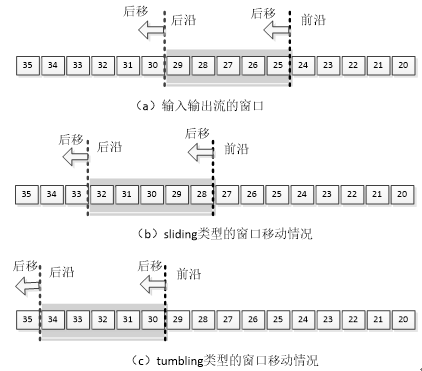
\includegraphics[width=5in]{Img/Chap_Application/Yu/operator.png}\\
	\caption{operator的窗口机制}\label{fig:operator}
\end{figure}
COStream对流中的数据访问采用窗口机制,窗口用前沿和后沿界定,前沿和后沿的距离就是当前operator执行时可操作的输入、输出缓冲区的大小,它由window中的参数确定。COStream中窗口类型有两种:sliding和tumbling。sliding代表滑动窗口类型,这种窗口有peek,pop和push操作,一般用于输入流;而tumbling则代表翻转窗口类型,只有push和pop操作,该种类型窗口既可以用于输出流也可以用于输入流。对于输入流主要的操作有pop和peek。pop操作删除输入流中最先到的token,并返回该token。peek(i)返回输入流中距离输入流窗口前沿的第i个token。对于输出流主要操作是push,push操作是将计算得到的token输出到输出流,对缓冲区的使用是从前沿到后沿的。operator一次执行完成后同时移动窗口的前沿和后沿。图\ref{fig:operator}(a)图描述COStream中的输入输出流的窗口示意图,图\ref{fig:operator}(b)和(c)分别表示如果(a)对应的窗口分别是sliding(5,3)和tumbling(5)时,一次operator执行完成后窗口的移动情况。


\subsubsection{Composite}
在面向过程编程的 C 语言中, 程序入口为 main 函数, 在函数中使用多种控制语句来编写程序。与之不同,在面向数据流编程的 COStream 语言,程序入口为 Composite Main,在其内部通过将不同 Operator 用Stream 变量进行连接来构造数据流图。

COStream定义的用于连接不同节点构造数据流图的Composite结构属于高层次(相对于operator)的复合结构,代表一个由一个或若干个operator组成的可重用的数据流图结构,它是对SDF图中可复用的子图的抽象。它既可以完整的表示一个数据流程序的数据流图结构,也可以作为子数据流图结构被调用。下面是一个略去细节信息的抽象 composite 例子,它表示输入的数据流 S 依次经过了3个 operator 的处理后,计算得到了输出流T。

\begin{algorithm}\label{algo:operator}
Composite Main(input S, output T)\{\\
 \hspace*{1 pc} S0 = first(S);\\
 \hspace*{1 pc} S1 = second(S0);\\
 \hspace*{1 pc} T  = third(S1);\\
\}
\end{algorithm}

composite主要由composite头部和composite体组成。composite头部表明该composite的输入输出边参数、composite参数以及composite的名称,COStream不支持匿名composite。composite的输入输出边参数是用来确定在生成SDF图时该composite结构所形成的子图与SDF图中其他节点的连接关系。composite参数主要是指composite结构在实际被调用时需要从调用处传入的参数,可以根据参数的情况决定composite最终子图的结构,另外该参数也可以在composite内部被使用。composite体主要有如下2部分组成:一部分是composite内部需要使用的变量的定义和一些相关的操作语句;另一部分是composite内部的子图结构,它由一个或若干operator组成,每个operator根据输入流、输出流的依赖关系连接成图,是composite的核心结构。Composite结构在编译阶段被扩展,经过编译数据流程序的数据流图子结构将被扩展成完整的数据流图。

\subsubsection{多输入多输出流的连接方式}

composite可以同时有多个输入多个输出边。下面的数据流程序例子反映了上述语言特点。

\begin{algorithm}\label{algo:operator}
composite M (output K,L,input G,H) \{		//1\\
 \hspace*{1 pc} stream<int x> I=O(G)\{\}			//2\\
 \hspace*{1 pc} stream<int x> J=P(H)\{\}			//3\\
 \hspace*{1 pc} stream<int x> K=Q(I;J)\{\}			//4\\
 \hspace*{1 pc} stream<int x>L=R(J)\{\}			//5\\
\}									//6\\
composite Main\{						//7\\
 \hspace*{1 pc} …\\
 \hspace*{1 pc} (stream<int x>C,stream<int x> D) = M(A,B)\{\}	//8\\
 \hspace*{1 pc} (stream<int x>E,stream<int x> F) = M(A,B)\{\}	//9\\
 \hspace*{1 pc} …\\
\}
\end{algorithm}

\begin{figure}[htbp]
	\centering
	% Requires \usepackage{graphicx}
	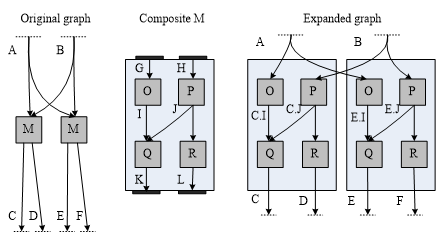
\includegraphics[width=1.0\textwidth]{Img/Chap_Application/Yu/multi.png}\\
	\caption{多输入多输出流连接方式}\label{fig:multi}
\end{figure}

图\ref{fig:multi}描述了行1至行9的程序片段所反映的数据流图调用、扩展过程:由Original graph扩展为Expanded graph。Original graph包含了2个composite结构M,第一个M将输入流A和B计算后得到输出流C和D,第二个M将输入流A和B计算后得到输出流E和F。行1定义了M的输入流为G和H,输出流为K和L。行8表示当M在Main中第一次被调用时,输入流和输出流发生实例化:G=A,H=B,K=G以及L=D。在Expand graph中M因为被调用2次而实例化成2份,所以M中的中间流I和J也被实例化为2份:C.I,C.J和E.I,E.J。这些子流图因被调用而实例化展开的过程在编译器编译时完成,经过编译后,数据流程序的流图结构将被扩展成完整的数据流图。

\subsubsection{pipeline 连接方式}

\begin{figure}[htbp]
	\centering
	% Requires \usepackage{graphicx}
	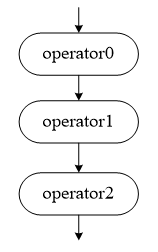
\includegraphics[width=0.25\textwidth]{Img/Chap_Application/Yu/pipeline.png}\\
	\caption{pipeline连接方式}\label{fig:pipeline}
\end{figure}

有时候我们会想要编写这样一种数据流结构: 每个 operator 的输入恰好是上一个 operator 的输出,即数据流在全局或局部保持单向传递,有时 operator 还可以复用。例如对应图\ref{fig:pipeline}中有3个 operator 的示例:

\begin{algorithm}\label{algo:costream}
Composite Main(input<int x> S0)\{\\
 \hspace*{1 pc} stream<int x>S1,S2,S3;\\
 \hspace*{1 pc} S1 = operator0(S0);\\
 \hspace*{1 pc} S2 = operator1(S1);\\
 \hspace*{1 pc} S3 = operator2(S2);\\
\}
\end{algorithm}

在这种情况下, 我们最关心的是输入流变量 S0和输出流变量 S3,而数据流变量S1,S2是多余的信息,实际上我们并不关心中间变量。在其它函数式编程语言中,我们可以使用 compose(组合)这个操作符来描述这种结构:

\begin{algorithm}\label{algo:costream}
operator3 = compose(operator0,operator1,operator2)\\
S3 = operator3(S0)
\end{algorithm}

等价于

\begin{algorithm}\label{algo:costream}
S3 = operator2(operator1(operator0(S0)))
\end{algorithm}

那么在COStream 数据流编程语言中, 有没有这种”串联”形式的组合结构呢?答案是有的, 这就是 pipeline 结构, 下面给出对应示例:

\begin{algorithm}\label{algo:costream}
Composite Main(input<int x> S0)\{\\
 \hspace*{1 pc} S3 = pipeline(S0)\{\\
 \hspace*{2 pc} add operator0();\\
 \hspace*{2 pc} add operator1();\\
 \hspace*{2 pc} add operator2();\\
 \hspace*{1 pc} \}\\
\}
\end{algorithm}

pipeline结构是由一串连续的composite调用组成,它们在pipeline结构中出现的先后顺序决定了它们在数据流图中的依赖关系。pipeline是单输入流单输出流,COStream规定能够在pipeline中被调用的composite也必须是单输入流单输出流。

\begin{algorithm}
  \caption{代码片段 A 和使用了 for/if 的代码片段 B 等价}
  \label{algo: pipeline}
  {\bf 代码片段 A}\\
  Composite Main(input<int x> S0)\{\\
    \hspace*{1 pc} S3 = pipeline(S0)\{\\
    \hspace*{2 pc} add operator0();\\
    \hspace*{2 pc} add operator1();\\
    \hspace*{2 pc} add operator0();\\
    \hspace*{2 pc} add operator1();\\
    \hspace*{2 pc} add operator0();\\
    \hspace*{2 pc} add operator1();\\
    \hspace*{1 pc} \}\\
  \}\\
  {\bf 代码片段 B}\\
  Composite Main(input<int x> S0)\{\\
    \hspace*{1 pc} S3 = pipeline(S0)\{\\
    \hspace*{2 pc} for(int i=0;i<3;i++)\{\\
    \hspace*{3 pc} if(i\%2==0)\{\\
    \hspace*{4 pc} add operator0();\\
    \hspace*{3 pc} \}\\
    \hspace*{3 pc} else\{\\
    \hspace*{4 pc} add operator1();\\
    \hspace*{3 pc} \}\\
    \hspace*{2 pc} \}\\
    \hspace*{1 pc} \}\\
  \}
\end{algorithm}

COStream引入add操作将operator和composite调用添加到pipeline中。 此外, pipeline 的结构体中支持使用 if 、for、while 语句等来控制 operator 的组合, 如算法\ref{algo: pipeline}所示,我们可以把代码片段 A 改写为代码片段 B,二者是等价的。





\subsubsection{splitjoin 连接方式}

\begin{figure}[htbp]
  \centering
  % Requires \usepackage{graphicx}
  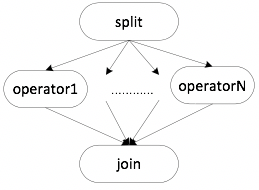
\includegraphics[width=0.5\textwidth]{Img/Chap_Application/Yu/splitjoin.png}\\
  \caption{splitjoin连接方式}\label{fig:splitjoin}
\end{figure}

除了 pipeline结构, 还有一种 splitjoin 结构用来描述数据流的分解与合并(图\ref{fig:splitjoin})。splitjoin结构由splitter、joiner以及一些composite调用组成,当一个流作为splitjoin结构的输入流时它被splitter分割,splitter根据splitjoin中composite调用情况产生一批满足相应条件的输出流作为不同的composite调用的输入流,这些composite调用的输出流作为joiner的输入流,joiner同样根据composite调用情况来合并各个输入流,将合并后产生的新的流作为joiner结点的输出,也是splitjoin结构的输出流。在splitjoin中splitter主要有两种方式:

\begin{itemize}	
  \begin{figure}[htbp]
    \centering
    % Requires \usepackage{graphicx}
    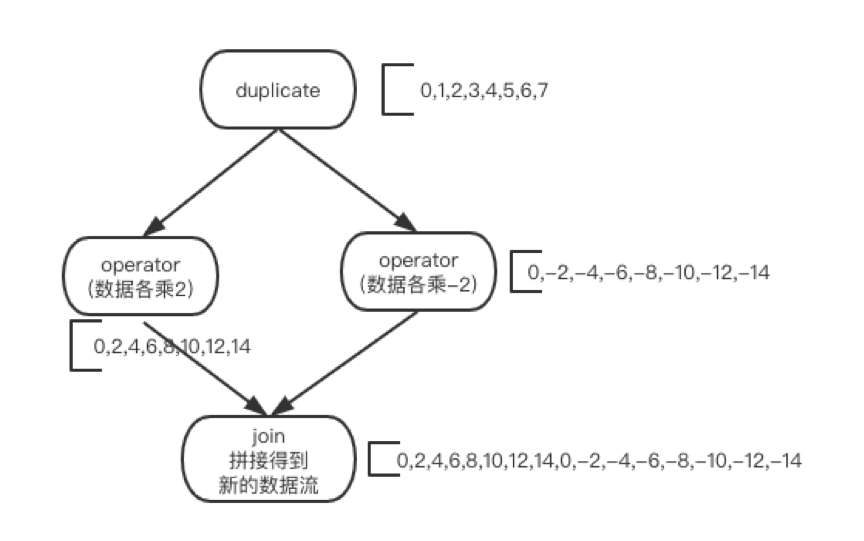
\includegraphics[width=0.8\textwidth]{Img/Chap_Application/Yu/duplicate.png}\\
    \caption{splitjoin-duplicate示意图}\label{fig:duplicate}
  \end{figure}

  \item {\bf duplicate方式}:该方式下所有的composite调用将会有完全相同的输入流。如图\ref{fig:duplicate}所示:

  \begin{figure}[htbp]
    \centering
    % Requires \usepackage{graphicx}
    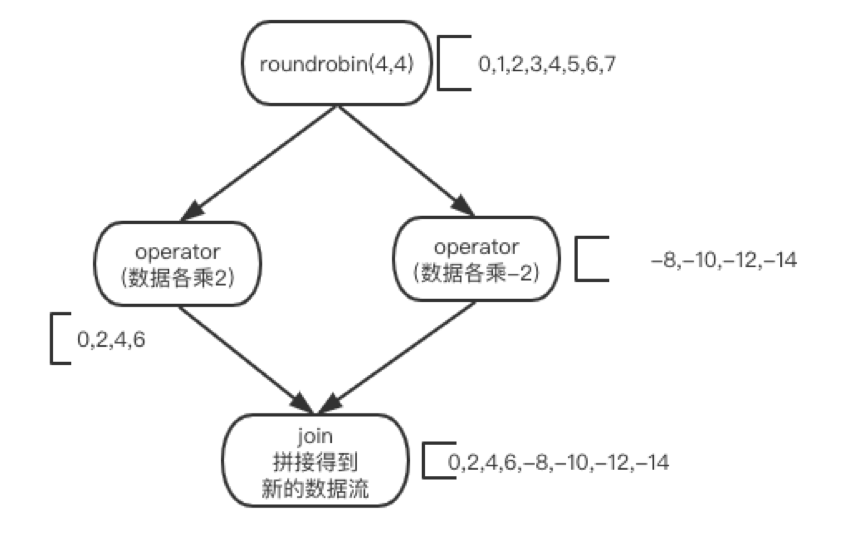
\includegraphics[width=0.8\textwidth]{Img/Chap_Application/Yu/roundrobin.png}\\
    \caption{splitjoin-roundrobin示意图}\label{fig:roundrobin}
  \end{figure}

  \item {\bf roundrobin(w1,…,wn)方式}:如图\ref{fig:roundrobin}所示,该方式下splitter将其输入流中的前w1个数据发送给第一个composite调用,接下来的w2个数据发送给第二个composite调用,以此类推,将最后的wn个数据发送给最后一个composite调用。对于joiner只有一种roundrobin方式。与pipeline结构类似,在splitjoin中调用的composite要求也是单输入流和单输出流的。
\end{itemize}

在COStream中splitter和joiner分别用关键字split和join表示,且可以和 pipeline 结构互相嵌套使用,下面是一个示例:

\begin{figure}[htbp]
  \centering
  % Requires \usepackage{graphicx}
  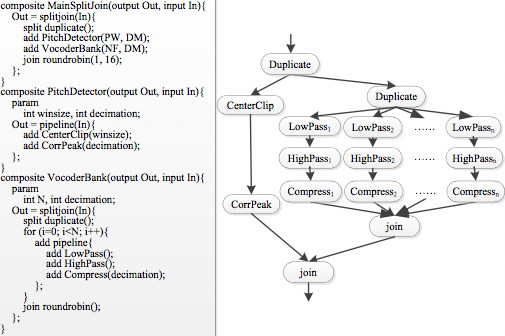
\includegraphics[width=1.0\textwidth]{Img/Chap_Application/Yu/vocodebank.png}\\
  \caption{vocodebank程序例子}\label{fig:vocodebank}
\end{figure}

图\ref{fig:vocodebank}的例子能够说明splitjoin和pipeline的层次性特点和使用特性。在图中左边部分是COStream的源码片段,右边是对应的数据流图。在本例中可以看到添加了层次性的结构有助于增加数据流程序编程的灵活性和可扩展性。另外,在splitjoin和pipeline中流能够被参数化,在本例composite VocodeBank中关于内置的pipeline调用次数可以有参数N来确定,通过N控制splitjoin结构的宽度,同样在pipeline中可以通过参数来控制pipeline的深度。

\subsubsection{内置 composite}

为了便于对文件操作,COStream对文件的I/O提供了内置composite支持,通过调用内置的文件I/O composite COStream可以完成对文件读写操作。FileReader和FileWriter是COStream为I/O提供的内置的composite接口。FileReader用于将文件中的数据读到流中,FileWriter是将流中的数据写到文件中。具体用法如下:

\begin{algorithm}\label{algo:costream}
stream<double x> A,B;			//1\\
A = FileReader(“data.bin”);		//2\\
FileWriter(B)(“result.txt”);
\end{algorithm}

行1表示将data.bin文件中的数据读入到数据流A中,行3表示将处理后输出的流B中的数据保存至文件result.txt。

此外,仍然存在许多常用能性 Composite有待于内置在COStream编程语言中, 实验室的全体师生会积极进行版本迭代,进一步改进和优化COStream的编程语言结构设计。 

\subsection{COStream 编译器框架}

\begin{figure}[htbp]
  \centering
  % Requires \usepackage{graphicx}
  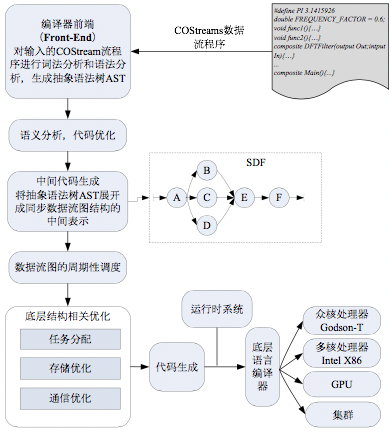
\includegraphics[width=0.8\textwidth]{Img/Chap_Application/Yu/compiler.png}\\
  \caption{COStream 编译器框架示意图}\label{fig:compiler}
\end{figure}

图\ref{fig:compiler}描述了COStream编译系统总体框架。COStream编译器的源语言为COStream数据流程序设计语言,目标语言根据目标结构不同生成不同底层语言,如C、C++(在x86平台上执行)和openCL(在 GPU 上执行)以及 Javascript(在跨平台的浏览器中执行)等,编译器通过调用底层语言编译器生成对应目标平台的可执行文件。下面详细介绍COStream编译系统的组成部分。

\begin{itemize}	
  \item {\bf 编译器前端}:编译器前端主要对COStream源程序进行分析,建立抽象语法树。对源程序的分析主要包括词法分析和语法性分析。在词法分析中,词法分析器从左到右地读构成源程序的字符流,把字符流分组为多个记号,记号是具有整体含义的字符序列。词法分析通常作为编译器的第一个阶段,产生记号序列,提交给语法分析使用。这里将词法分析作为语法分析的子程序来实现。当词法分析器收到语法分析器发出“取下一个记号”的命令时,词法分析器读入字符,识别出一个记号。COStream采用自底向上的语法分析过程。在语法分析中,将字符串或者记号划分为具有一定层次的多个嵌套组,每个嵌套组具有一个完整的含义。程序的层次性结构是通过递归规则来表达,在编译器中,语法分析器接受词法分析器提供的记号串,检查它们是否符合COStream的文法规则。如果文法匹配则通过规则建立语法树结点结构。源程序通过词语法分析最终将建立为一种由顶层语法树节点表示的层次性抽象语法树结构。COStream采用Lex和Yacc词语法生成器生成词语法分析器。

  \item {\bf 语义分析和代码优化}: 编译器对经过词语法分析形成的抽象语法树进行语义分析。语义分析是对COStream数据流程序进行类型检查以及为代码生成阶段收集类型信息。语义检查负责检验每个操作符的操作数是否满足源语言的说明。在该阶段除语义检查外还对源程序代码做机器无关优化。优化是在保持源程序语义的基础上减少代码占用空间,删除不必要的操作,降低程序运行时开销。为了提升程序的性能COStream实现了常见的机器无关优化,如常量传播和冗余代码删除等。该阶段得到最佳抽象语法树。
  \item {\bf 中间代码生成}: COStream编译器以同步数据流图作为中间表示,在该阶段分析编译器前端得到的抽象语法树,得到数据流程序中的composite调用关系和stream依赖关系,利用这两种关系将抽象语法树进行深层次的展开,得到一个只有operator通过stream相连的完整的数据流图的抽象语法树结构,利用此时的抽象语法树生成SDF图,该SDF图是编译器后续操作的基础。另外,在该阶段还需要对SDF图中的各个节点的工作量进行估计,确定SDF图中各个actor的负载情况。
  \item {\bf 数据流图的周期性调度}: 编译器根据中间表示的数据流图结构采用单出现调度策略 (Single Appearance Schedule,SAS) 得到静态平衡数据流图。编译器根据程序中各个operator的peek、pop和push率决定初态和稳态调度阶段的各个actor的执行次数,为后续的优化和代码生成提供依据。
  \item {\bf 底层结构相关优化}: 编译器根据不同底层系统结构特性,对COStream程序进行与底层结构相关的优化,主要从计算任务分配、存储优化和通信优化等方面对程序进行优化,在开发并行性的同时减小相应的开销,使数据流程序在执行时能够充分利用底层系统的资源,提高程序的执行效率。COStream主要针对X86、GPU和多核集群等目标系统做编译优化。在第\ref{section:x86}节中具体介绍面向X86共享多核架构下的相关优化。
  \item {\bf 代码生成}: 根据底层结构相关优化的结果和后端的体系结构以及目标代码的特性,设计最终目标代码的生成框架,生成高效的可并行代码。
  \item {\bf 运行时系统}: 运行时系统是采用目标语言编写的静态链接库,包括支持目标代码运行所需要通信库和函数库,为代码生成提供辅助支持。
  \item {\bf 底层编译器}: 编译器将生成的目标底层代码交由底层语言编译器编译生成指定目标平台的可执行文件,完成整个编译过程。
  
\end{itemize}

\subsection{面向 X86 多核集群的 COStream 编译优化} \label{section:x86}

随着多核处理器平台日趋复杂,数据流程序的并行编译优化工作变得更加困难,其问题主要包括多处理器核的并行调度和对主存的访问延迟。针对数据流程序根据共享存储多核架构的结构特点,构造出高吞吐量低延迟的软件流水线调度,主要分为任务划分、阶段赋值、流水线执行三个步骤。

\subsubsection{任务划分}

任务划分是在避免浪费处理器核的计算能力以及确保各处理器核间的任务负载均衡的基础上,使用合适的划分算法将数据流任务划分到合适的核上。任务划分的目的是根据数据流图(SDF图)中计算节点的负载和计算节点间的依赖关系构造高吞吐量低延迟的软件流水线调度,以最大化底层系统资源利用率。数据流程序要想充分利用系统资源就必须充分合理地利用其自身的数据并行性、任务并 行性和流水线并行性。在软件流水线调度中,流水线的启动间隔(Initiation Interval,II)是指相邻两次循环迭代进入流水线的时间间隔,II越小意味着吞吐率越大。任务划分的目的就是要最小化II。在软件流水中II是由流水线中各资源的处理时间决定,在X86中,资源主要是处理器核,那么影响程序最终执行性能的主要因素就是划分的负载均衡情况。

在进行任务划分前,需要对SDF进行预处理,包括扩大调度和融合相邻计算节点。扩大调度指的是以相同的扩大因子,成倍扩大每个计算单元稳态调度阶段的执行次数,这样可以减少同步开销对程序性能的影响。相邻计算节点的融合是指将两个独立且在数据流图中相邻的计算节点融合为一个计算单元。相邻

计算单元融合操作保证了两个计算单元不会被分配到不同的处理器核上调度,这能够减少通信开销对程序的影响; 但是过度的融合操作会减少数据流图的计算单元,可能导致任务划分阶段负载的不均衡。相邻计算单元融合算法的关键在于如何判断是否某对相邻计算单元进行融合。首先,被融合的计算单元必须是单输入单输出的,这是由于过多的通信边将导致复制分裂后计算单元间过多的通信开销;其次,因为存在状态计算单元不能进行数据并行调度,所以不对相应状态计算单元进行融合操作。对于满足上述两个条件的相邻节点,根据两者通信量之和以及融合后的计算量,当通信计算比大于某个阈值时,将其合并为一个计算单元。

在对SDF图进行预处理优化后,在此基础上采用划分算法来进行任务划分。COStream 任务划分采取以负载均衡为目标同时最小化同步通信开销的分配策略。负载均衡的目的是为了保证流水线在满状态时各个核上的有效计算时间是相等的,核间因相互等待而产生的空闲时间将会小,II就会小,处理核利用率就高,系统的吞吐量就大。同时,因为SDF中计算节点之间有数据依赖,为了保证数据访问的局部性最小化同步通信延迟,在任务划分时应该尽可能地将有依赖关系的计算节点分配在一个核上以最大程度地减少核间通信边的数量。文献比较了常见的任务划分和分配策略,常见的分配策略主要包括有循环分发分配策略、亲和性分配策略和贪心分配策略等。综合COStream程序运行时存在的问题及常见任务分配策略,COStream选择以负载均衡为目标同时最小化通信开销的 K路图划分算法(MultilevelK-way Partitioning,MKP)。COStream采用Metis提供的接口实现MKP算法为SDF图作任务分配。由于MKP作为通用的图划分算法,没有充分结合数据流程序自身存在的各种并行性其结果并不能很好地满足程序运行的要求,COStream在MKP划分结果的基础上根据数据流程序的特点进行了进一步优化,提出复制分裂算法,图9描述了复制分裂算法的基本流程。复制分裂算法根据 MKP 划分结果的负载平衡情况,利用了SDF图中无状态的计算节点存在的数据并行性,对无状态的计算节点做分裂,增大任务并行性,将分裂产生的不同副本分配到不同的划分子集中,降低计算节点粒度,使不同划分的负载达到平衡。经过实验分析看到,COStream在X86环境下平衡因子设为1.5时能够得到较理想的结果,其中平衡因子指的是划分中负载最大的与最小的比值。

\subsubsection{阶段赋值}

\begin{algorithm}
  \caption{阶段赋值算法}
  \label{algo:stage}
  输入:SDF图G(V,E),图G计算单元到核的映射actorProcMap\\
  输出:图G计算单元到阶段号的映射actorStageMap\\
  1.	topologicalOrder = topologicalTrav();\\
  2.	for all actor v in topologicalOrder do\\
  3.	  \hspace*{1 pc} int maxStage = 0; int stage;\\
  4.	  \hspace*{1 pc} for all actor u which is a parent of v do\\
  5.	    \hspace*{2 pc} if (actorProcMap[u] != actorProcMap[v]) then\\
  6.	    \hspace*{3 pc}   stage = actorStageMap[u] + 1;\\
  7.	    \hspace*{2 pc} else\\
  8.	    \hspace*{3 pc}   stage = actorStageMap[u];\\
  9.	    \hspace*{2 pc} endif\\
  10.	    \hspace*{2 pc} if ( stagemaxStage) then\\
  11.	    \hspace*{3 pc}   maxStage = stage ;\\
  12.	    \hspace*{2 pc} endif\\
  13.	  \hspace*{1 pc} end for\\
  14.	  \hspace*{1 pc} actorStageMap[v] = maxStage;\\
  15.	 end for
\end{algorithm}

阶段赋值是为了确定数据流计算节点分配到流水线的哪个阶段执行,在考虑各个计算节点之间的依赖关系的基础上,在空间维度上和时间维度上指定各个计算节点的相对计算顺序以满足计算节点间数据依赖关系。算法\ref{algo:stage}用伪代码描述了计算单元的阶段赋值算法,其以目标程序对应的数据流图和任务划分结果作为输入。对于数据流程序,其数据流图的有向边表示计算单元间的数据传输。算法首先构造数据流图中计算单元节点的拓扑排序以满足计算单元数据读写规则;然后以拓扑序列依次访问计算单元,根据数据读写节点是否被划分到同一个处理器核上确定计算单元的流水调度阶段值。算法1描述了阶段赋值的过程。首先,对数据流图G(V, E)进行拓扑排序;其次,按照数据依赖关系依次访问所有的actor,对u∈ V,令maxStage为0,遍历u的每个输入边(v,u)∈E,如果v和u在不同处理核上,则u的阶段号stageu = stagev + 1;否则u的阶段号stageu = stagev。如果stageu > maxStage,则更新maxStage。在遍历完u的每条边后,以maxStage作为u的阶段号

\subsubsection{流水线执行}

\begin{figure}[htbp]
  \centering
  % Requires \usepackage{graphicx}
  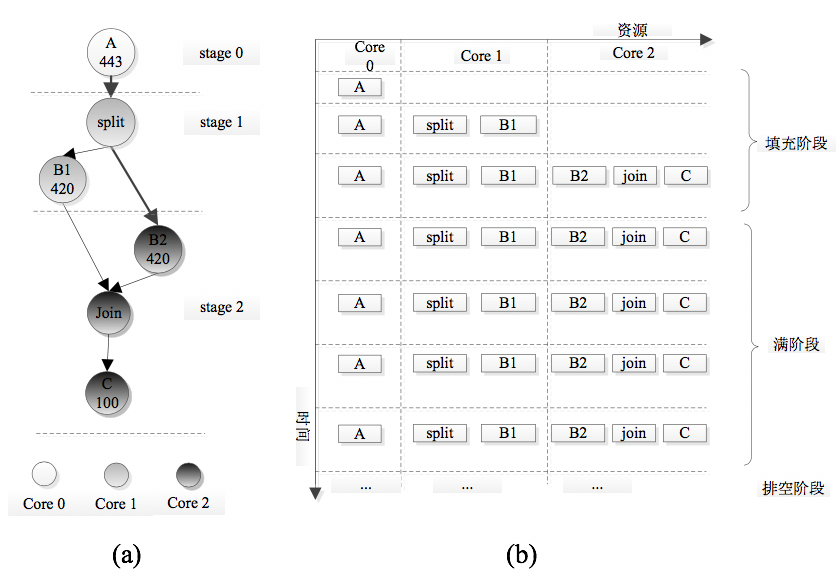
\includegraphics[width=1.0\textwidth]{Img/Chap_Application/Yu/streamline.png}\\
  \caption{(a)任务划分和阶段赋值的例子 (b)图(a)对应的软件流水执行过程}\label{fig:streamline}
\end{figure}

流水线执行过程分为三个阶段,分别是填充阶段、满阶段以及排空阶段。图\ref{fig:streamline}给出了任务划分、阶段赋值和软件流水调度执行的一个例子。初始SDF图 有A、B和C这3个计算节点,在任务划分阶段将B复制分裂成两个计算单元B1和B2,同时引入了split和join两个计算节点。经过任务划分后,计算单元A被分配到处理器核core0,split和B1被分配到core1,B2、join和C被分配到core2上。图\ref{fig:streamline}(a)给出了经过阶段赋值后各个计算单元的阶段值,完成了软件流水的构造。图\ref{fig:streamline}(b)给出了对应的软件流水调度执行过程,程序启动时流水线处于填充阶段,各个核上的计算节点按照其阶段值从小到大的顺序启动执行,当所有的计算节点都启动时,流水线进入满阶段;在流水线满阶段,所有的计算节点都进行周期性的迭代执行,由于任务划分阶段基本实现了不同计算核上的负载均衡,此时核间同步开销小,资源利用率高,系统的吞吐率达到最大;在流水线调度的排空阶段,程序开始相继结束计算节点的执行,各个核的计算节点按照阶段值从小到大的顺序结束其周期性的迭代,等到所有的计算节点结束其稳态调度后,整个程序终止并释放运行时占有的各种资源。

\subsubsection{性能评估}
为了对COStream编译系统面向X86架构的编译优化进行全面的性能评估和分析,选取了11个多媒体领域常见的算法作为测试程序用COStream数据流编程语言实现作为COStream编译器的输入。
\begin{figure}[htbp]
  \centering
  % Requires \usepackage{graphicx}
  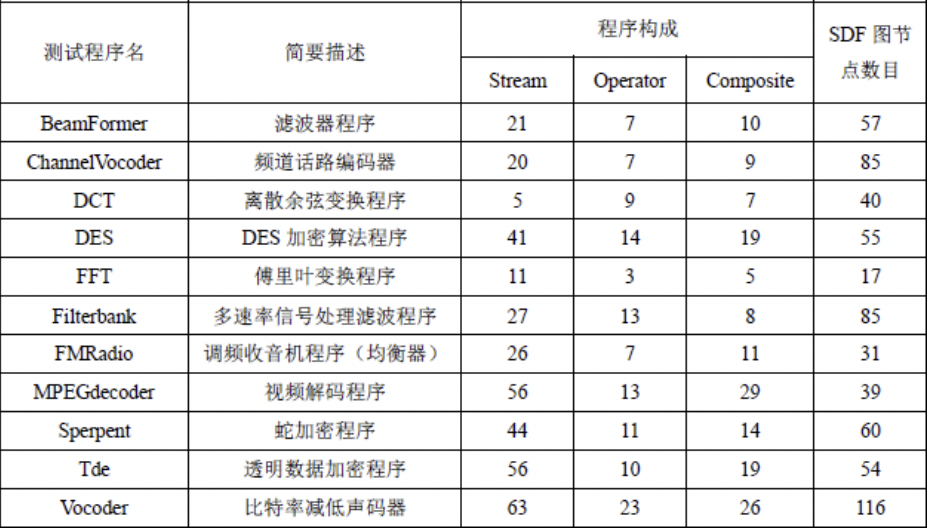
\includegraphics[width=1.0\textwidth]{Img/Chap_Application/Yu/x86benchmark.png}\\
  \caption{用于测试的数据流程序信息}\label{fig:x86benchmark}
\end{figure}

图\ref{fig:x86ratio}给出了测试程序经过COStream编译后在目标环境上执行的加速比。从图中可以看出,每个程序执行加速比随着处理核的数目增多而增加,基本呈现一个线性的加速情况。
\begin{figure}[htbp]
  \centering
  % Requires \usepackage{graphicx}
  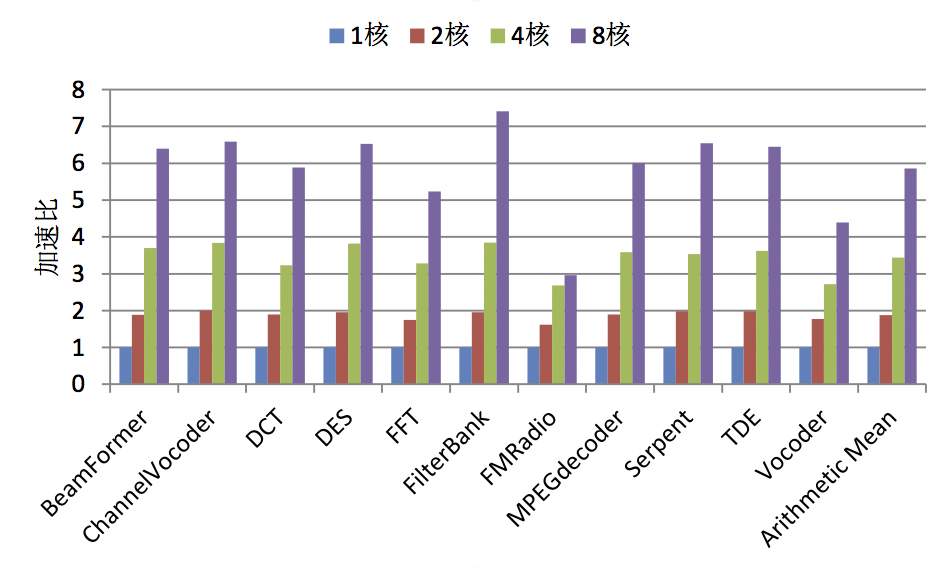
\includegraphics[width=0.8\textwidth]{Img/Chap_Application/Yu/x86ratio.png}\\
  \caption{测试代码在X86上达到的加速比}\label{fig:x86ratio}
\end{figure}

通信与同步比衡量了测试程序的有用计算和时间开销之间的比例,在一定程度上反应了程序的性能。在X86环境下采用的是软件流水调度策略,各个并行线程在软件流水调度的每次执行阶段中需要进行一次同步操作,COStream采用sense-reversing barrier[ ] 做核间的同步,保证不同核上的actor间的数据依赖关系能够满足。图\ref{fig:x86computeSync}给出了各个测试程序在8个核上的运行时计算同步时间分布。从图\ref{fig:x86computeSync}可以看出,FMRadio和Vocoder的计算同步比不太理想,同步开销太大,导致加速比较低,对于其他的测试程序计算同步比都能够达到较高水平,程序的加速比也较为理想。

\begin{figure}[htbp]
  \centering
  % Requires \usepackage{graphicx}
  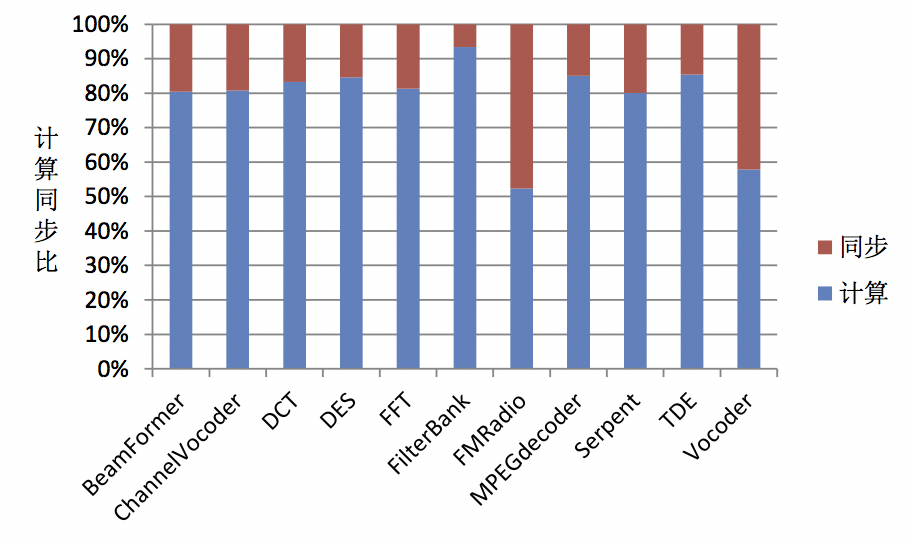
\includegraphics[width=0.8\textwidth]{Img/Chap_Application/Yu/x86computeSync.png}\\
  \caption{测试程序在8核上运行的计算同步比}\label{fig:x86computeSync}
\end{figure}

\subsection{面向 CPU 和 GPU 异构多核集群的 COStream 编译优化}

目前,各种新型的高性能体系结构不断涌现,以传统处理器CPU与图形处 理器GPU协同工作模式来构建异构硬件平台逐渐成为一种新型的并行处理方 式。CPU/GPU异构集群是由多个服务器节点组成的集群,其中每个节点封装多 核CPU与一定数量的GPU。CPU/GPU异构集群相对通用CPU集群在计算、访存与通信方面存在很大的差异性,这给研究人员带来了难度。 

COStream在异构集群的数据流程序的编译优化上,提出并实现了面向 CPU/GPU混合架构的数据流程序任务划分方法和多粒度调度策略,包括任务的分类处理、GPU端任务的水平分裂和CPU端离散任务的均衡化,构造了软件流水调度,经过编译优化生成OpenCL目标代码。

GPU在大规模数据的并行方面有很大的优势,但GPU间的通信开销却相当巨大,任务划分目的主要是保证各服务器节点的计算负载均衡、通信开销最小化,以及在单个节点上,充分发挥CPU逻辑控制与串行计算特点以及GPU计算密集性优势,同时保证 CPU 多核间负载均衡和不同GPU间数据通信开销最小化。COStream在异构集群的数据流程序的编译框架中的任务划分算法主要分为任务划分预处理任务划分与调度。

\subsubsection{任务划分预处理}
该阶段主要分成两个步骤:一是引入扩大因子,二是任务的分类处理。引入扩大因子,即计算节点执行次数整体扩大,在各个应用程序中,各计算节点的执行次数远远小于GPU可并行执行的规模,采用执行次数的整体扩大的方法,增大各个计算节点的工作量,从而充分利用GPU的并行计算单元;扩大因子的上限由三个因素决定:主存大小(Host Memory)、GPU存储空间(Device Memory)和GPU缓冲区分配机制。

CPU端允许扩大倍数为N1,则
\begin{equation}
  N_1 \leq M_{CPU} / M_{CPUSumneeded} \label{eq:2.1}
\end{equation}

其中,MCPU表示主存可用空间的大小,MCPUSumneeded表示CPU端所有任务未扩大前所需的存储空间总和。

GPU端允许扩大的倍数为N2,N2需满足公式\ref{eq:2.2}和公式\ref{eq:2.3}。
\begin{equation}
  N_2 \leq M_{GPU} / M_{GPUSumneeded} \label{eq:2.2}
\end{equation}

其中,$M_{GPU}$表示GPU可用的存储空间,$M_{GPUSumneeded}$表示GPU端所有任务未扩大前所需的存储空间总和。

\begin{equation}
  N_2 \leq M_{GPU} / M_{GPUSumneeded} \label{eq:2.3}
\end{equation}

其中,$M_{GPUmaxbuffer}$表示GPU每次允许分配缓冲区的最大值,$M_{GPUmaxneeded}$表示GPU端所有任务未扩大前各需存储空间的最大值。

在同时满足公式\ref{eq:2.1}、公式\ref{eq:2.2}、公式\ref{eq:2.3}的前提下,选取合适的扩大因子为来保证GPU端任务有足够的计算量,并充分利用GPU计算资源。同时,引入扩大因子的过程间接地减少了CPU线程的同步次数,从而降低了应用程序整体的同步开销。

任务的分类处理,该步骤根据任务是否具有可并行性以及相应通信开销的大小将其分配到GPU或CPU上去运行,充分利用CPU与GPU各自的优势,同时降低整体程序的通信量。COStream数据流程序中,计算节点有两种状态:有状态(Stateful)和无状态(Stateless)。状态为Stateful的结点表示该计算结点连续两次迭代运算间存在数据依赖,两次迭代运算不可并行执行;状态为Stateless的结点则与之相反,多次换代运算之间互相独立,可并行执行。数据流程序任务的分类处理,目标是根据计算节点的计算特点,将计算节点分配到适合的计算平台上进行计算,在分类的过程中,既要考虑该计算任务是否具有可并行性,即是否为状态是Stateless的结点,同时也要考虑GPU间高额的通信开销,减小异构平台间的数据通信量。任务分类首先判断SDF图中各个计算节点的状态,将Stateless计算节点划分到GPU端,Stateful计算节点划分到CPU端。接着考虑异构平台间的通信开销,调节边界结点。对于划分到GPU端的Stateless结点,如果其父结点为Stateful结点,并且其子结点为Stateful结点,那么初步分类的结果就会带来大量的GPU间的数据通信,从而产生巨大的通信开销,影响数据流程序的整体性能,因此任务初步分类完成后,需要将此类计算节点微调到CPU端。

\subsubsection{任务划分}
基于GPU/CPU混合架构的数据流程序任务划分包括两部分内容——GPU端任务的水平分裂(GPU Tasks Horizon Splitting, GTHS)和CPU端离散任务均衡化(CPU Disperse Tasks Balancing, CDTB)。

对于任务划分,它既要满足负载均衡,又要降低通信开销,常用的针对SDF图的划分方法有METIS划分工具、K路图划分方法等。METIS划分与K路划分方法都满足负载均衡和减小通信开销的目标,由于GPU与GPU间数据通信开销的巨大,导致这两种划分方法对应用程序的整体执行效率提高不显著。

针对上述问题,GTHS算法利用任务的并行性将其均衡分裂到各GPU,以防止GPU与GPU间高额的通信开销影响数据流程序的整体性能。算法\ref{algo:gths}描述了GPU端任务水平分裂的具体实现过程,该方法主要分为两个阶段完成:一是GPU端actor的分裂,完成任务的分类处理和扩大因子的引入后,划分到GPU端的任务各自的迭代计算具有很高的并行性,但针对一些特殊的应用程序,其GPU端任务间的数据访问对前一次的运行结果有依赖性,对于这种特殊类型的应用程序不进行GPU端任务的水平分裂,而将分配到GPU端的任务均由一个GPU计算完成;该划分方法针对GPU端任务间数据访问对前一次的运行结果无依赖性的应用,遍历分配到GPU端的各actor,修改各actor的稳态执行次数,并创建M个新actor(M为GPU的个数减1),将该actor复制给M个新创建的actor(称该actor为新创建的M个actor的模板结点,新创建的M个actor为该actor的复制结点),并修改对应新结点的名字(行1-12);二是对应的新结点连接,actor分裂完成后,新创建的actor是离散的,将各离散的新创建的actor对应连接起来,形成新的连通的SDF图(行13-42)。依次遍历每一个新创建的actor,如果其模板actor的父结点是GPU端actor,则该新创建的actor的模板结点的父结点在上一阶段也进行了水平分裂,那么将该新创建的actor与其模板actor的父结点的相应复制结点连接起来;如果其模板actor的父结点是CPU端actor,则其模板actor的父结点在上一阶段未进行水平分裂,那么将该新创建的actor与其模板actor的父结点直接连接起来(行14-27);如果其模板actor的子结点是GPU端actor,则该模板结点的子结点在上一阶段也进行了水平分裂,那么需要将该新创建的actor与其模板actor的子结点的相应复制结点连接起来;如果其模板actor的子结点是CPU端actor,则该模板actor的子结点在上一阶段未进行水平分裂,那么需要将该新创建的actor与其模板actor的子结点直接连接起来(行28-41)。如图\ref{fig:3.1}所示为数据流程序GPU端任务水平分裂的结果示意图,图\ref{fig:3.1}(a)为任务的分类结果,计算节点A和计算节点F为CPU端结点计算节点B、C、D、F为GPU端结点;图\ref{fig:3.1}(b)为GPU端任务水平分裂结果,其中,计算节点A和计算节点F为CPU端结点,计算节点B1、C1、D1和E1划分到GPU0,计算节点B2、C2、D2和E2划分到GPU1,计算节点B3、C3、D3和E3划分到GPU2。

\begin{breakablealgorithm} \label{algo:gths}
  \caption{GPU端任务水平分裂算法}
  {\bf Input: GPUNode[ ], SDF graph}\\
  {\bf Output: new SDF graph}\\
  1 for all actor v in GPUNode[] do\\
  2   \hspace*{1 pc} v.executions /= GPUNumber;\\
  3   \hspace*{1 pc} int NewActorNumber = GPUNumber – 1;\\
  4   \hspace*{1 pc} int index = 1;\\
  5   \hspace*{1 pc} multimap mapActor2NewActor;\\
  6   \hspace*{1 pc} for int i = 0; i < NewActorNumber; ++i do\\
  7   \hspace*{2 pc} Actor m = CreateNewActor(v);\\
  8   \hspace*{2 pc} m.name += itoa(index);\\
  9   \hspace*{2 pc} mapActor2NewActor.insert(v,m);\\
  10  \hspace*{2 pc} ++index;\\
  11  \hspace*{1 pc} end for\\
  12 end for\\
  13 for all actor u in GPUNode[] do\\
  14  \hspace*{1 pc} if(IsGPUNode(u.parent))then\\
  15  \hspace*{1 pc} int index = 1;\\
  16  \hspace*{1 pc} for ;index < GPUNumber;++index do\\
  17  \hspace*{2 pc} Actor a = FindNewActor(u,index);\\
  18  \hspace*{2 pc} Actor b= FindNewActor(u.parent,index);\\
  19  \hspace*{2 pc} a.parent = b;\\
  20  \hspace*{1 pc} end for\\
  21  \hspace*{1 pc} else\\
  22  \hspace*{1 pc} int index = 1;\\
  23  \hspace*{1 pc} for ; index < GPUNumber; ++index do\\
  24  \hspace*{2 pc} Actor a = FindNewActor(u,index);\\
  25  \hspace*{2 pc} a.parent = u.parent;\\
  26  \hspace*{1 pc} end for\\
  27  \hspace*{1 pc} end if\\
  28  \hspace*{1 pc} if(IsGPUNode(u.child))then\\
  29  \hspace*{1 pc} int index = 1;\\
  30  \hspace*{1 pc} for ;index < GPUNumber;++index do\\
  31  \hspace*{2 pc} Actor a = FindNewActor(u,index);\\
  32  \hspace*{2 pc} Actor b= FindNewActor(u.child,index);\\
  33  \hspace*{2 pc} a.child = b;\\
  34  \hspace*{1 pc} end for\\
  35  \hspace*{1 pc} else\\
  36  \hspace*{1 pc} int index = 1;\\
  37  \hspace*{1 pc} for ; index < GPUNumber; ++index do\\
  38  \hspace*{2 pc} Actor a = FindNewActor(u,index);\\
  39  \hspace*{2 pc} a.child = u.child;\\
  40  \hspace*{1 pc} end for\\
  41  \hspace*{1 pc} end if\\
  42 end for
\end{breakablealgorithm}


\begin{figure}[htbp]
  \centering
  % Requires \usepackage{graphicx}
  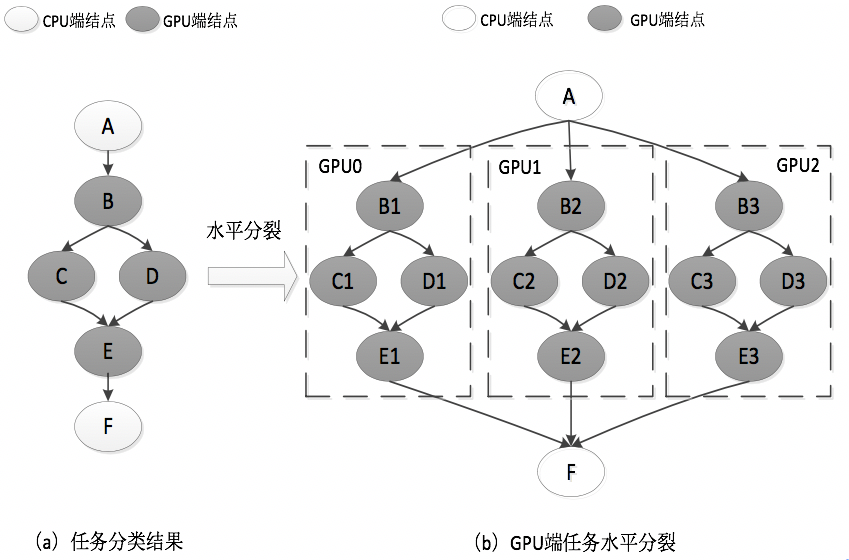
\includegraphics[width=0.8\textwidth]{Img/Chap_Application/Yu/3-1.png}\\
  \caption{GPU端任务水平分裂示意图}\label{fig:3.1}
\end{figure}


GPU/CPU混合架构平台下,GPU端任务的水平分裂完成了GPU端任务的划分,而传统的任务划分方法对任务分类处理后分配到CPU端的各个离散结点未进行划分处理,均由一个CPU核控制计算,如果该CPU核的工作量过大时就会影响整个程序的执行效率。数据流程序CDTB算法针对这些CPU端的离散结点,结合复制分裂算法,选择合适CPU核,采用贪心的思想,均衡地将各计算结点分成若干个划分并将各划分映射到相应的CPU核上,保证各CPU核的负载均衡并提高各CPU核的利用率。基于GPU/CPU混合架构的数据流程序CPU端离散任务的均衡化过程主要包括以下三个阶段:

\begin{itemize}	
  \item {\bf CPU核数的确定}:图3.2为CPU核数确定过程的流程示意图。分别计算CPU端任务总的执行时间CPUTime、GPU端任务总的计算时间GPUTime以及数据流程序总的通信时间CommTime,如果CPUTime小于GPUTime和CommTime的最大值,选择CPU的核数为1,即分配到CPU端所有actor均由一个CPU核控制执行;如果CPUTime大于GPUTime和CommTime的最大值且分配到CPU端的actor个数为1,该actor的状态为stateful即该actor不可进行分裂,则选择CPU的核数为1;如果分配到CPU端的actor个数大于1或者存在工作量较大的状态为stateless的actor,根据公式3.1计算出应用程序执行时所需要的CPU核数NCPUcore;如果所求得的CPU核数大于系统可用的核数,则设置所需的CPU核数为系统可用的核数。通过CPU核数的确定,充分利用系统的计算资源,减小系统计算资源的浪费。

  \item {\bf CPU端工作量相对较大且状态为stateless的actor复制分裂}: 根据CPU端所有actor总的工作量CPUTotalWork和计算出所需的CPU核数NCPUcore,结合公式\ref{eq:3.2}求得理论上分配给每个核的最大工作量MaxTotalWork,遍历CPU端的状态为stateless的actor,根据工作量估计求出该actor的工作量大小,如果其工作量大于MaxTotalWork,则利用复制分裂算法对该actor进行复制分裂操作,将新生成的actor与其模板actor的父结点和子结点连接以保证SDF的连通性,经过多次反复的复制分裂操作使CPU端每个状态为stateless的actor的工作量都小于MaxTotalWork。
  
  \begin{equation}
    MaxTotalWork = CPUTotalWork/N_{CPL} \label{eq:3.2}
  \end{equation}

  \item {\bf CPU端各离散的actor与CPU核间的映射}: 该过程采用贪心的思想,遍历CPU端actor并根据工作量估计计算出该actor的工作量,选择当前各自总工作量最小的CPU核,将该actor划分到当前总工作量最小的CPU核上,完成该actor与CPU核映射。算法\ref{algo:cpureflect}描述了CPU端离散任务均衡化具体过程的实现细节,该方法适合于CPU端计算成为软件流水调度过程中数据流程序整体效率瓶颈的情况。根据公式3.1和公式3.2分别计算出该应用程序所需的CPU核数NCPUcore和每个CPU核理论最大的总的工作量MaxTotalWork,遍历CPU端所有状态为stateless的actor结点,针对工作量workvalue大于MaxTotalWork的actor,通过CreateNewActor函数对该actor进行分裂操作并将新创建的actor与其模板actor的父结点和子结点连接(行1-11)。遍历所有CPU端actor,选择当前总的工作量估计最小的CPU核并完成该actor与该CPU核的映射(行12-17)。
\end{itemize}

\begin{algorithm}
  \caption{CPU Disperse Tasks Balancing Algorithm}
  \label{algo:cpureflect}
  Input: CPUNode[]\\
  Output: mapActor2Partition(actor:partition)\\
  for( all actor v in CPUNode[] ) \{\\
    \hspace*{1 pc} int workvalue = CalculateWorkValue(v);\\
    \hspace*{1 pc} if(!DetectiveActorState(v) \&\& workvalue > MaxTotalWork)\{\\
    \hspace*{2 pc} int number = workvalue / MaxTotalWork;\\
    \hspace*{2 pc} for(int i = 0; i < number; ++i) \{\\
    \hspace*{3 pc} Actor u = CreateNewActor(v);\\
    \hspace*{3 pc} u.parent = v.parent;\\
    \hspace*{3 pc} u.child = v.child;\\
    \hspace*{2 pc} \}\\
    \hspace*{1 pc} \}\\
  \}\\
  for( all actor w in CPUNode[] )\{\\
    \hspace*{1 pc} int workvalue = CalculateWorkValue(w);\\
    \hspace*{1 pc} int index = FindMinWorkvalueCore();\\
    \hspace*{1 pc} UpdateWorkvalue(index);\\
    \hspace*{1 pc} mapActor2Partition(w:index);\\
  \}
  \end{algorithm}

\subsubsection{阶段赋值}
基于GPU/CPU混合架构的数据流程序优化框架采用软件流水调度方式,主要解决了软件流水调度过程中的三个问题:

\begin{itemize}	
  \item {\bf 线程同步问题}:在软件流水调度过程中,每个线程执行完各自的计算任务后,都需要进行一次同步操作,保证各个线程处于同一调度阶段,虽然该同步开销比硬件调度方式下的同步开销小,但由于计算任务的工作量过小或者处理器核数的增加都有可能带来同步开销的增大,从而影响了应用程序的执行效率。该优化框架引入扩大因子,成倍的扩大计算任务的稳态执行次数,增大各个计算任务的工作量,使计算任务多次计算后,同步一次,从而大大地减小了程序的同步操作数,增加了计算同步比,同时也充分利用了GPU/CPU混合架构下GPU高度并行计算的优势,提高了数据流程序的执行效率。

  \item {\bf 负载均衡问题}: 软件流水调度过程中,负载均衡是影响应用程序整体执行效率的重要因素。在GPU/CPU混合架构系统平台下,由于GPU与CPU计算能力的不对等,如果各个线程的负载不均衡,则会带来多个线程忙等的现象,增加程序的同步开销。该优化框架通过GPU端任务水平分裂算法和CPU端离散任务均衡化算法,实现了GPU端计算、CPU端计算和异构通信的相对均衡,同时降低了应用程序的通信量。
  
  \begin{equation}
    MaxTotalWork = CPUTotalWork/N_{CPL} \label{eq:3.2}
  \end{equation}

  \item {\bf 通信开销问题}: 在GPU/CPU混合架构中,异构通信占用软件流水调度的一个阶段,达到软件流水满状态,即计算任务稳态执行阶段,CPU端任务的计算、GPU端任务的计算以及CPU与GPU间的数据通信是并行执行的,高额的通信开销也会降低应用程序的执行效率。该优化框架采用任务分类方法,结合任务的计算特点,完成任务的分类,同时也降低异构的通信开销;GPU端任务的水平分裂,将GPU端任务均衡分裂到各GPU,避免了GPU与GPU间的高额通信,达到降低通信开销的目的。
\end{itemize}

经过GPU端GTHS算法和CPU端CDTB算法的任务划分,SDF图中的actor均被划分到对应的计算单元上运行,挖掘状态为stateful类型的结点的流水线并行性,构造软件流水线调度,使得状态为stateful的结点连续两次迭代计算,结点计算和数据传输都可以重叠执行,需要确定各结点被流水调度执行时的阶段号,即进行阶段赋值。

\begin{algorithm}
  \caption{基于GPU/CPU混合架构的阶段赋值}
  \label{algo:gpucpu}
  Input: SDFgraph, CPUNode[],GPUNode[], mapActor2Partition(actor:partition)\\
  Output: mapActor2Stage(actor:stage)\\
  TopologyOrderofActors = TopologyTravSDF();\\
  int MaxStage = 0;\\
  int tempStage;\\
  for all actor v in TopologyOrderofActors \{\\
    \hspace*{1 pc} for all actor u which is parent of v \{\\
    \hspace*{2 pc} if((IsCPUNode(v) \&\& IsCPUNode(u)) || IsGPUNode(v) \&\& IsGPUNode(u))\{\\
    \hspace*{3 pc} if(mapActor2Partition[v] == mapActor2Partition[u])\{\\
    \hspace*{4 pc} tempStage = mapActor2Stage[u];\\
    \hspace*{3 pc} \}else\{\\
    \hspace*{4 pc} tempStage = mapActor2Stage[u] + 1;\\
    \hspace*{3 pc} \}\\
    \hspace*{2 pc} \}else\{\\
    \hspace*{3 pc} tempStage = mapActor2Stage[u] + 2;\\
    \hspace*{2 pc} \}\\
    \hspace*{2 pc} if(tempStage > MaxStage)\{\\
    \hspace*{3 pc} MaxStage = tempStage;\\
    \hspace*{2 pc} \}\\
    \hspace*{1 pc} \}\\
    \hspace*{1 pc} mapActor2Stage[v] = MaxStage;\\
  \}
\end{algorithm}

算法\ref{algo:gpucpu}描述了面向GPU/CPU混合架构的数据流程序阶段赋值过程。对SDF图进行拓扑排序以满足数据的读写规则(行1),依次遍历拓扑排序中的各actor,如果该actor与其父结点同在CPU端或同在GPU端,并且属于同一个划分,那么该actor阶段号与其父结点阶段号相同;如果该actor与其父结点同在CPU端或同在GPU端,但是不属于同一个划分,那么该actor阶段号等于其父结点阶段号加1;如果该actor与其父结点不同在CPU端或GPU端,那么该actor阶段号等于其父结点阶段号加2(行4-21),因为该actor与其父结点不同在CPU端或不同在GPU端则会产生通信,数据通信在软件流水调度过程中需要占用一个阶段号。图\ref{fig:gpucpu}所示为基于GPU/CPU混合架构的阶段赋值结果,其中,actor A、B、C为CPU端结点,actor D、E、F、G、I为GPU端结点,在CPU端,actor A为一个划分,actor B和C属于同一个划分,actor A的阶段号为0,actor B与actor A都是CPU端结点,但不属于同一划分,根据算法\ref{algo:gpucpu},actor B的阶段号为actor A的阶段号加上1;actor C和actor B都是CPU端结点,并且属于相同的划分,因此,actor C的阶段号等于actor B的阶段号;actor D与actor C分配在不同的平台,即不同在GPU或CPU,actor D的阶段号为actor C的阶段号加上2,因为actor C与actor D的数据通信需要占用一个阶段号,由于GPU的并行规模比较丰富,实验中将分配到GPU并且连通的结点划分同一个阶段执行。


\begin{figure}[htbp]
  \centering
  % Requires \usepackage{graphicx}
  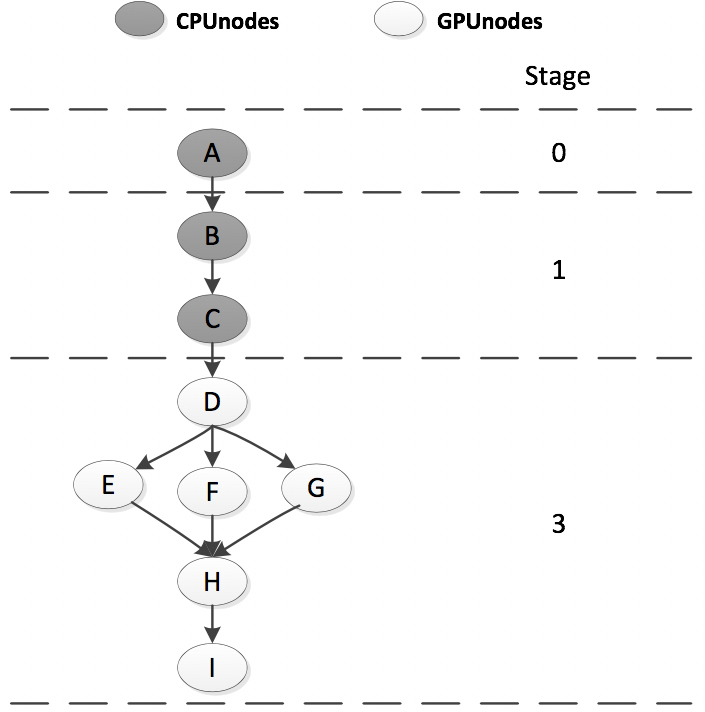
\includegraphics[width=0.8\textwidth]{Img/Chap_Application/Yu/gpucpu.png}\\
  \caption{基于GPU/CPU混合架构的阶段赋值}\label{fig:gpucpu}
\end{figure}

在三块NVIDIA Tesla C2050、两块四核CPU为混合架构系统结构上进行测试,如图。选取9个数字多媒体领域的典型算法作为测试程序。

\begin{figure}[htbp]
  \centering
  % Requires \usepackage{graphicx}
  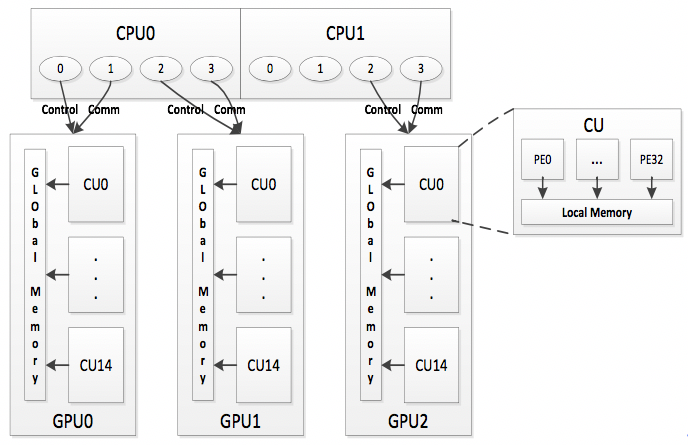
\includegraphics[width=0.8\textwidth]{Img/Chap_Application/Yu/fusion.png}\\
  \caption{混合架构系统结构}\label{fig:fusion}
\end{figure}

图\ref{fig:gm-commu}和图\ref{fig:gths-metis}显示了比较GPU端任务水平分裂算法与通用METIS划分算法的通信量以及执行时间的结果。可见在GPU/CPU混合架构平台下GTHS算法的执行效果优于METIS划分方法。

\begin{figure}[htbp]
  \centering
  % Requires \usepackage{graphicx}
  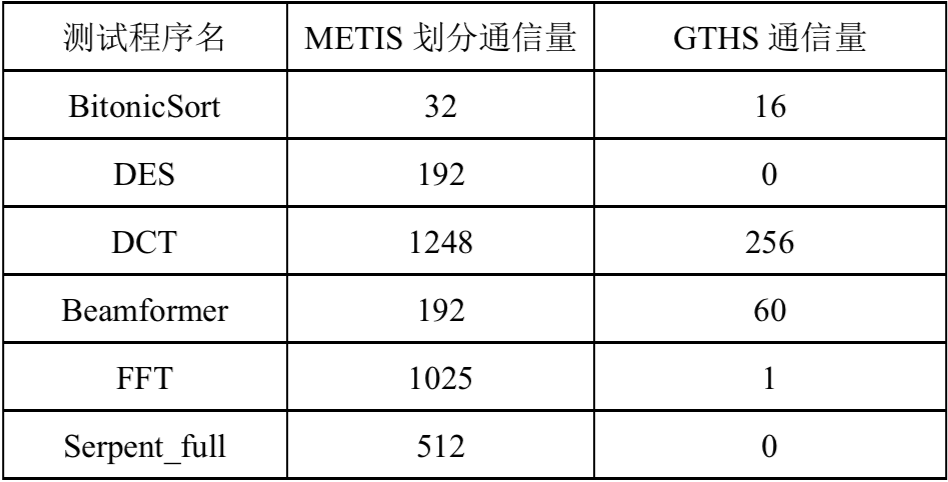
\includegraphics[width=0.8\textwidth]{Img/Chap_Application/Yu/gths-metis-commu.png}\\
  \caption{GTHS与METIS划分通信量比较}\label{fig:gm-commu}
\end{figure}

\begin{figure}[htbp]
  \centering
  % Requires \usepackage{graphicx}
  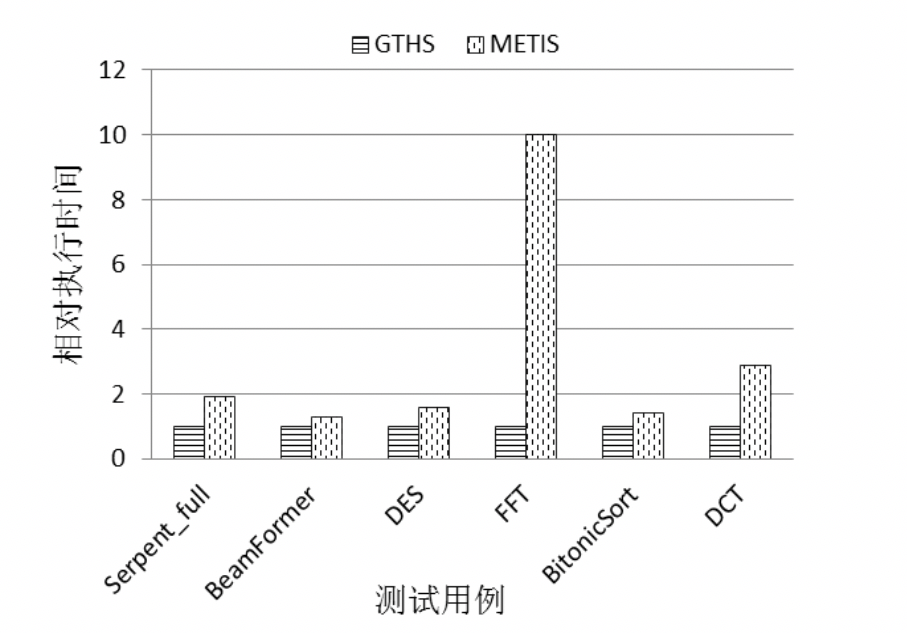
\includegraphics[width=0.8\textwidth]{Img/Chap_Application/Yu/gths-metis.png}\\
  \caption{GTHS与METIS划分执行性能比较}\label{fig:gths-metis}
\end{figure}

对于CPU端任务较重的情况采用CDTB方法进行任务划分,比较CPU端离散任务均衡化算法与传统CPU端单核计算的执行时间。可见CDTB方法更适合于CPU端任务较重且状态为stateful的actor的计算量较小的应用程序。

\begin{figure}[htbp]
  \centering
  % Requires \usepackage{graphicx}
  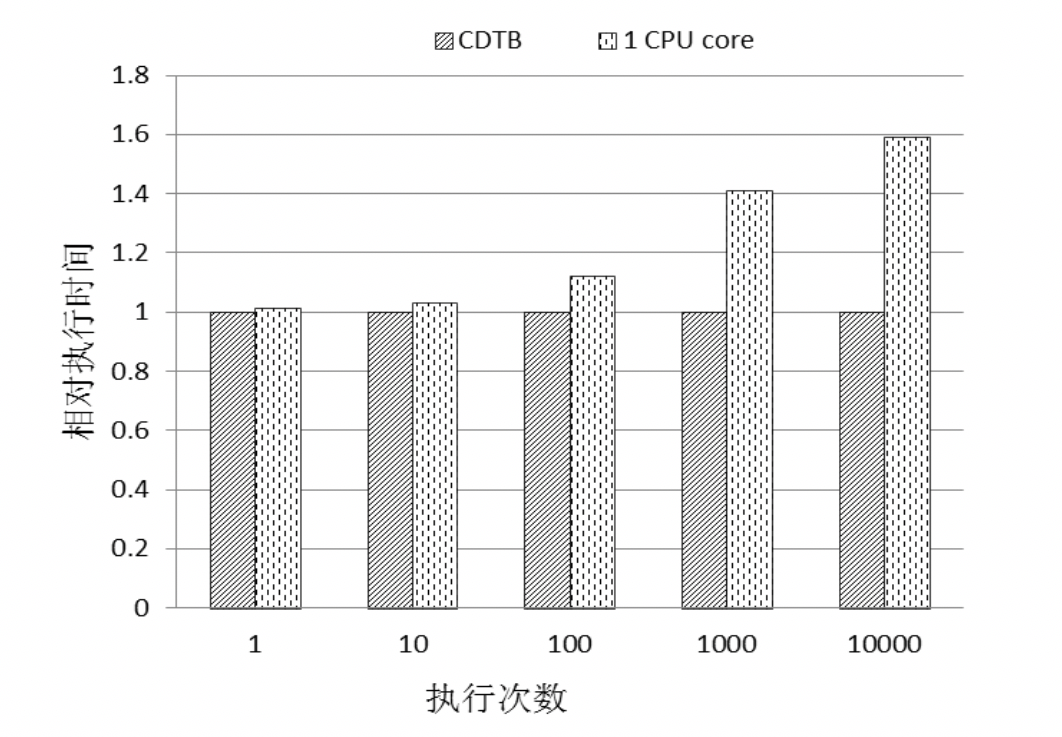
\includegraphics[width=0.8\textwidth]{Img/Chap_Application/Yu/bitonicsort.png}\\
  \caption{BitonicSort采用CDTB算法与传统CPU端单核计算的性能比较}\label{fig:bitonicsort}
\end{figure}

在GPU/CPU混合架构平台上,采用CPU与GPU协作计算的模式,充分发挥各计算单元的优势,CPU负责控制主程序的流程和串行计算,准备GPU端计算所需的相应的数据并将其传输给GPU,充分利用GPU进行高效的并行计算。图5.4为数据流程序分别采用CPU单核和1个GPU协作计算的模式与CPU单核计算并执行1000次的性能比较示意图,测试程序Beamformer中存在大量离散的状态为stateful的结点,导致执行过程中产生大量的CPU与GPU的数据通信,高额的数据通信开销使程序的性能只提高6.8,相对加速效果不明显。而对于测试程序FFT和ChannelVocoder,程序内部的通信开销相对GPU的计算开销很小,充分利用了GPU强大的并行计算规模,所以加速效果显著。

\begin{figure}[htbp]
  \centering
  % Requires \usepackage{graphicx}
  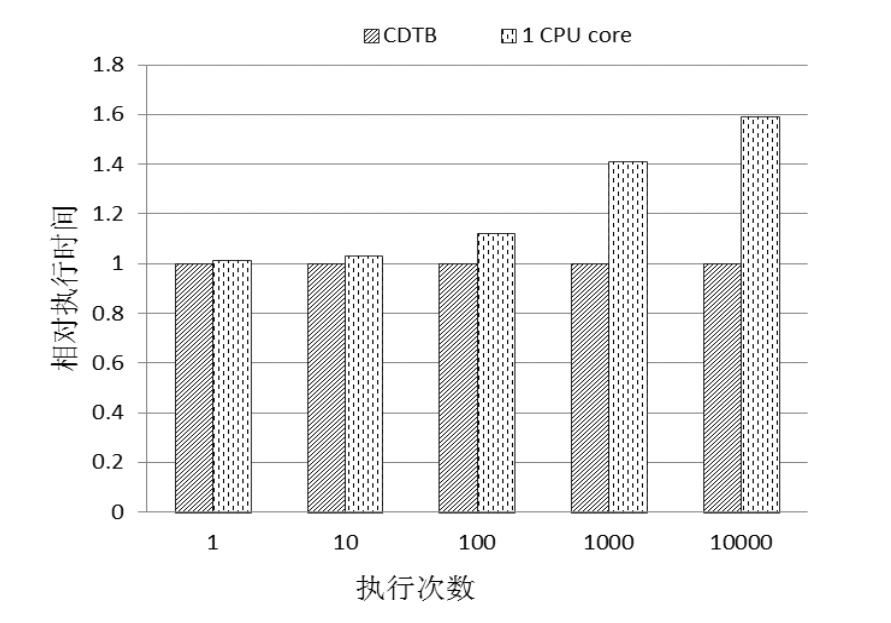
\includegraphics[width=0.8\textwidth]{Img/Chap_Application/Yu/cpugpu-cpu.png}\\
  \caption{CPU与GPU协作计算相对CPU单核的性能比较}\label{fig:cpugpu-cpu}
\end{figure}

图\ref{fig:3gpu-1gpu}所示为数据流程序分别采用三个GPU与一个GPU并执行1000次的执行性能的比较示意图。从图中可以看出,对于测试用例BeamFormer和BitonicSort,CPU端任务计算量较重,远远大于GPU端的运行时间,采用三个GPU进行并行计算,相对于采用一个GPU计算的加速效果不明显。而对于测试用例Serpent\_full和DES,CPU端任务计算量较轻,远小于GPU端任务的计算时间,采用三个GPU并行计算的加速效果比较显著。

\begin{figure}[htbp]
  \centering
  % Requires \usepackage{graphicx}
  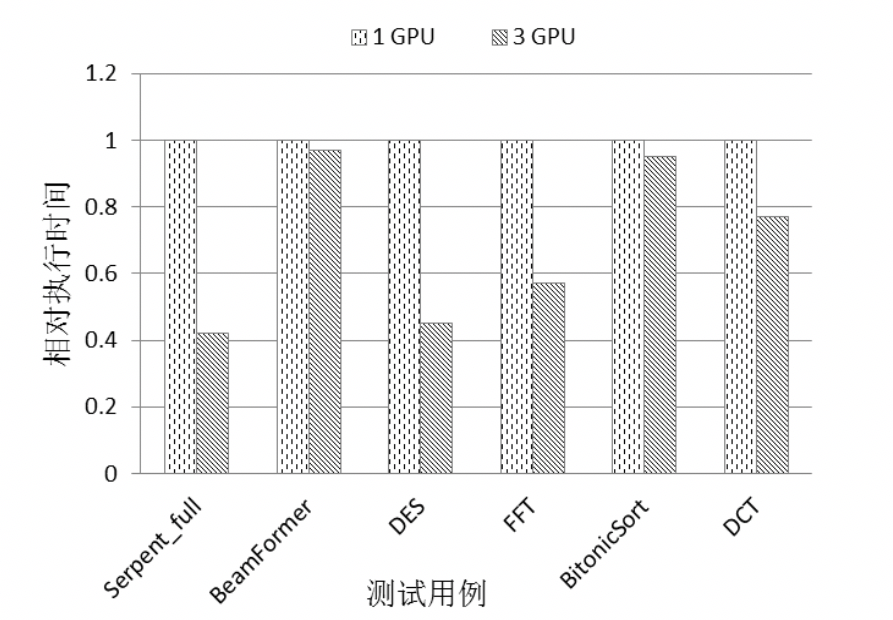
\includegraphics[width=0.8\textwidth]{Img/Chap_Application/Yu/3gpu-1gpu.png}\\
  \caption{三个GPU与一个GPU执行性能比}\label{fig:3gpu-1gpu}
\end{figure}

\subsection{基于 COStream 的深度学习程序开发实例}
\subsubsection{全连接神经网络的并行化分析与设计}
全连接神经网络由全连接层组成,全连接层的每一个神经元都与上一层的所有神经元相连,用来将该层之前提取到的特征综合起来,本质上是多层感知机。

为处理基于MNIST数据集的手写数字识别问题,设计一个深度为4,每个隐藏层宽度为20的全连接神经网络模型,其输入层宽度为数据集中单张图片的像素数784,输出层宽度为10,依次对应手写图片为数字0到9预测概率。图\ref{fig:dnn}表示的是整个全连接神经网络模型的架构。

\begin{figure}[!t]
\centering
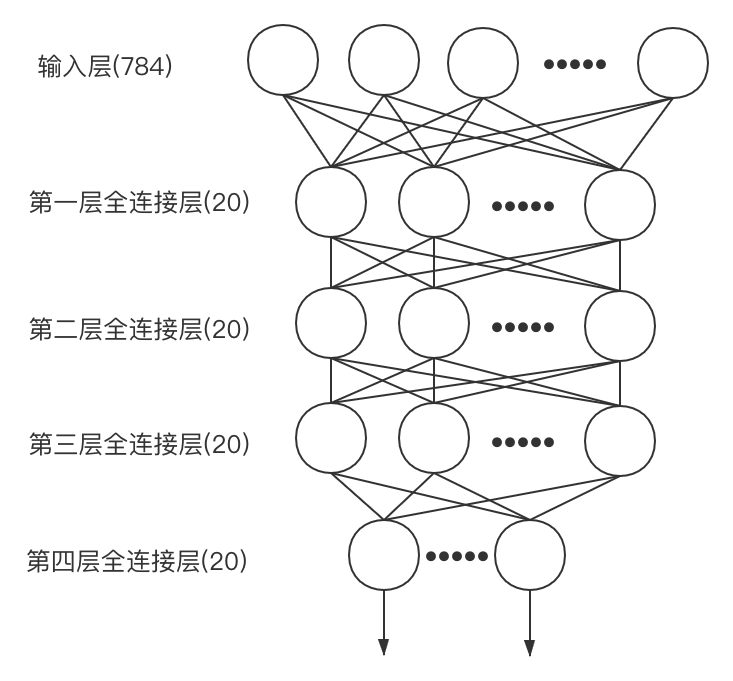
\includegraphics[width=0.5\textwidth]{../img/Chap_Application/Yu/dnn.png}
\caption{3隐层每层20节点的全连接神经网络}
\label{fig:dnn}
\end{figure}

正向传播计算过程其实是多个函数的复合,图\ref{fig:dnn}描述了本模型中函数如何复合在一起。假设模型中每一层对应的函数依次为$f^{\left (1 \right )}$、$f^{\left (2 \right )}$、$f^{\left (3 \right )}$、$f^{\left (4 \right )}$,则复合成一条$f\left ( x \right )= f^{\left (4 \right )}\left ( f^{\left (3 \right )}\left ( f^{\left (2 \right )}\left ( f^{\left (1 \right )}\left ( x \right ) \right ) \right ) \right )$的计算链,其中x代表输入层的输入,相邻层之间存在数据依赖,形成流水线,而隐藏层、输出层层内的各节点间没有数据依赖关系,即每一层内是由许多可并行操作的节点构成,每个节点执行一个从向量到标量的计算。因此,在上层所有节点完成运算输出结果后,下层中的各个节点可以同时用流入的结果数据展开本层的计算,在数据流模型中以一个图节点代表神经网络模型中的神经元的方式来表示这种层内的数据并行关系。

反向传播计算过程也是多个函数的复合,利用链式求导法则,逐层计算参数梯度,上层内的节点依赖下层各节点参数梯度,还依赖于正向传播时该节点的输入值,同样可以用图节点代表神经元的方式对该层进行数据并行处理。最终,根据误差更新参数。

正向传播和反向传播各层间在时间维度上是串行关系,可以用数据流编程模型提供的软件流水线并行方式进行处理。

对于模型中的参数,由于深度学习模型计算除依赖于上一个计算节点输出的数据流,还依赖于网络模型中的随着计算迭代更新的参数,因此各层节点的参数需要定义在程序中composite结构外的全局区域内,作为全局变量使用。

四层全连接神经网络正向传播的并行化实现包括四个模块,第一个是输入层模块,第二个是隐藏层模块,第三个是输出层模块,第四个是正反向传播过渡模块。

\begin{enumerate}
\item 输入层模块负责处理数据的输入并在operator的init代码块中定义各层参数的初始化方法。
\item 隐藏层模块对应神经网络中的三层隐藏层,隐藏层的实现需要构造层composite和节点composite两种composite,层composite利用COStream语句splitjoin中的duplicate重复分发上层流出的数据到节点composite。由于splitjoin语句只支持单输入单输出数据流,因此将正向传播时各个节点的执行结果同参数一样也保存在composite结构外的全局区域,用于在反向传播时进行参数梯度的计算。
\item 输出层模块负责处理上层传入的数据并得到0到9十个数字的预测概率值,同样以splitjoin对10个输出节点的composite进行调用。
正反向传播过渡模块负责计算损失函数的误差,并将其传递给反向时的输出层以供计算参数梯度,之后进入反向传播过程。

\end{enumerate}

四层全连接神经网络反向传播的并行化实现包括三个模块,第一个是反向输出层模块,第二个是反向隐藏层模块,第三个是参数更新模块。

\begin{enumerate}
\item 反向输出层模块连接着正向传播时的过渡层模块,过渡层模块将损失函数误差计算完毕后继续传递给反向输出模块。同样构造层composite和节点composite两种composite,其中节点composite计算本层节点的参数关于损失函数的偏导数以及本层在正向传播中的输入关于损失函数的偏导数;层composite使用COStream语句splitjoin通过duplicate重复分发过渡层模块误差数据流,向节点composite传递误差。
\item 反向隐藏层节点和反向输出层节点的操作基本一致。
\item 参数更新模块负责对隐藏层和输出层内的参数更新。参数更新操作必须保证原子性,即一次更新全部参数,不能只更新部分参数,所以模块中由一个单独composite负责更新全部参数,同时在参数更新前计算实际的改变量。

\end{enumerate}

\subsubsection{LeNet-5 卷积神经网络的并行化分析与设计}

当前设计的LeNet-5卷积神经网络模型参照经典LeNet-5卷积神经网络模型,并在其基础上做了结构的微调,当前卷积神经网络模型拥有一个输入层、三个卷积层,两个池化层、两个全连接层和一个输出层,输入层以MNIST数据集中的单张图片作为输入。相对于经典LeNet-5卷积神经网络模型,当前模型增加了一层全连接层,并将全连接层的层内节点数缩减至20,其余结构均保持不变。图\ref{fig:cnn}是该模型的结构示意图。

\begin{figure}[!t]
\centering
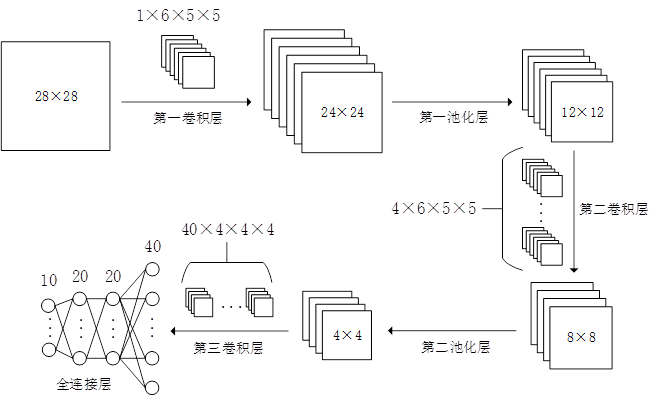
\includegraphics[width=0.5\textwidth]{../img/Chap_Application/Yu/cnn.png}
\caption{LeNet-5卷积神经网络模型的结构示意图}
\label{fig:cnn}
\end{figure}

在图\ref{fig:cnn}中,模型输入的是一个单通道的28×28大小的图片数组数据,第一卷积层被设定为用6组每组一个5×5大小的卷积核进行单步卷积计算,卷积完毕并经ReLU激励后得到6个24×24大小的输出数据,经第一次2×2最大池化后得到6个12×12的输出数据,第二卷积层被设定为用4组每组6个5×5大小的卷积核进行单步卷积计算,完毕后经ReLU激励得到4个8×8大小的输出数据,再经第二次2×2最大池化后得到4个4×4大小的输出数据,第三卷积层被设定为用40组每组4个4×4大小的卷积核进行单步卷积计算,得到一个有40个数据的一维向量,这40个数据将是全连接层的输入数据,两个全连接层均有二十个节点,输出层则有10个节点,两个全连接层和一个输出层在经历了加权求和并以Sigmoid激励函数激励的过程后,最终由输出层输出节点对应数字的预测概率值

在LeNet-5卷积神经网络模型的正向传播过程中,各个卷积层的每一组的每一个卷积核在对输入的数据进行卷积处理时,互相之间均不存在数据依赖,因此可以用数据并行的方式将其在数据流编程模型中进行表示。池化层每次的输入的都是一个以三维数组表示的多个二维矩阵,其中各个二维数据的池化过程互不相关,所以可以同样用数据并行的方式对其进行表示。全连接层的并行化方法已经在本小节第一部分描述,各层的不同节点间也是用数据并行的方式表示。

在LeNet-5卷积神经网络模型的反向传播过程中,误差先通过全连接层进行传播,此过程的并行化方法同本小节第一部分所述一致,当误差传递至卷积层时,卷积层节点需要经过三个过程完成计算过程,分别是: 
\begin{enumerate}
\item 用传入的误差与正向传播时输入该层节点的数据做卷积操作的方式得到卷积核weight权重参数的梯度。
\item 用对误差矩阵各项求和的方式得到卷积核组的bias偏置参数的梯度。
\item 用转置后的卷积核矩阵与用零填充过的误差矩阵做卷积操作的方式得到在正向传播时位于该层上层的节点所需要的误差。
\end{enumerate}
这三个过程都只需传入的误差或是正向传播时临时保存的各层输出值,其中任一过程所需数据不依赖于其他过程,对此可采用数据并行的方式进行并行化。

误差在经过卷积层的反向传播处理后,输出的是反向池化层所需的误差,此时误差和池化层正向传播的输出结果维数一致,都是以三维数组形式表示的多个二维矩阵,其中每个二维矩阵在反向池化层中需要进行一次上采样过程,并将采样结果与ReLU激励函数对池化层输入数据的偏导数做一次Hadamard积运算,才能得到下一个反向卷积层所需的误差值。这个过程没有数据依赖,同样可以用数据并行的方式,对三维数组中的每个二维矩阵同时进行处理。

将整个LeNet-5卷积神经网络模型的正向传播和反向传播连接起来看,各层间都是需要上层处理完成后传入处理结果才能执行本层,彼此间有着单向的数据依赖关系,因此可以用流水线并行的方式,将每层的处理过程抽象为流水线的一个阶段,到达并行化的目的。

对于模型中的参数值,由于正反向传播过程均需要使用,所以各个卷积层的卷积核参数和卷积层组参数以及全接连层各节点的参数均作为全局变量保存在composite体外的全局区域中,全局区域同样还临时保存着正向传播过程中所有模块中各层的输出结果以供反向传播过程计算使用。

LeNet-5卷积神经网络正向转播过程包括七个模块,分别是输入层模块、卷积层模块、池化层模块、卷积与全连接过渡模块、全连接模块、输出层模块和正反向传播过渡模块。
输入层模块负责获取28×28大小的图片数组数据并传递给下层,同时要在模型的第一次执行前初始化所有卷积核的参数以及全连接层节点的参数,此过程通过设计inlayer comoposite结构,在inlayer composite内部的init语句块内以满足高斯分布的随机值初始化各个参数,在work语句块内读取图片数组数据。

\begin{enumerate}
\item 输入层模块

输入层模块负责获取28×28大小的图片数组数据并传递给下层,同时要在模型
的第一次执行前初始化所有卷积核的参数以及全连接层节点的参数,此过程通过设计inlayer comoposite结构,在inlayer composite内部的init语句块内以满足高斯分布的随机值初始化各个参数,在work语句块内读取图片数组数据。

\item 卷积层模块

卷积层模块负责对输入层中的三维矩阵进行卷积操作,此时把三维矩阵看成是多通道的二维矩阵,其第一维度通道数,即二维矩阵的个数与每组卷积核的个数一致,组内的各个卷积核以一一对应的方式对各个二维矩阵进行卷积操作,每组多个卷积核的单次卷积操作完成后,需要将其卷积结果相加并加上该组bias偏置参数得到带激励的输出,再经ReLU激励函数激励后得到最终的输出结果。整个层的卷积过程在COStream中可以借助两层splitjoin结构的嵌套进行描述,最外层的conv\_layer composite中用pipeline的形式分别对卷积组conv\_group composite和conv\_bias composite进行add操作,conv\_bias comoposite负责对每组各个卷积核卷积后的输出结果进行求和,并对求和结果进行ReLU激励,conv\_group composite负责调用conv\_kernel composite进行卷积计算。conv\_layer composite以splitjoin的duplicate调用形式对上层传入的三维矩阵进行复制,复制后的各个三维矩阵分别流入不同组的conv\_goup composite中,调用conv\_group composite时传入group\_index用于定位全局区域中该组对应的bias偏置参数。conv\_group composite则以splitjoin的roundrobin调用形式对传入的三维矩阵进行切割,切割成的多个二维矩阵分别流入对应的conv\_kernel composite中,以上就是卷积层两次splitjoin嵌套中的输入数据变化情况。conv\_group composite在调用conv\_kernel composite时则要传入group\_index和kernel\_index,用以定位在全局区域中卷积核的weight权重参数,传入size参数,用以确定被卷积的矩阵的大小。图\ref{fig:cnn_conv_layer}是卷积层模块中各个composite间的结构关系示意图。

\begin{figure}[!t]
\centering
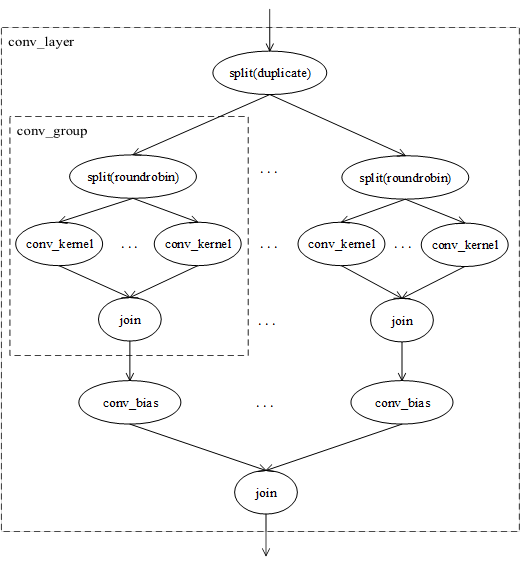
\includegraphics[width=0.5\textwidth]{../img/Chap_Application/Yu/cnn_conv_layer.png}
\caption{卷积层模块中composite间的结构关系示意图}
\label{fig:cnn_conv_layer}
\end{figure}

\item 池化层模块

池化层模块负责将输入的三维矩阵按不同通道分成多个二维矩阵,并分别以2×2大小的池化区域进行最大池化,池化过程同样需要两个composite结构,一个是pool\_layer composite,一个是pool composite,pool\_layer composite内部使用split的roundrobin调用形式对单通道池化过程的pool composite进行add操作,将不同通道的二维矩阵数据发送至不同的pool composite进行池化操作。池化层的pool\_layer composite在对pool composite进行add操作时,不需要传递表示位置顺序的index参数,因为splitjoin语句中的split和join以相同的操作顺序对被add的composite进行数据分发和合并,即split切割后的第一批数据被对应节点处理完毕后所生成的数据,仍会被join第一个处理,因此COStream中的splitjoin操作保证了数据间的相对顺序不变。图\ref{fig:cnn_pooling_layer}是池化层模块中两类composite的结构关系。

\begin{figure}[!t]
\centering
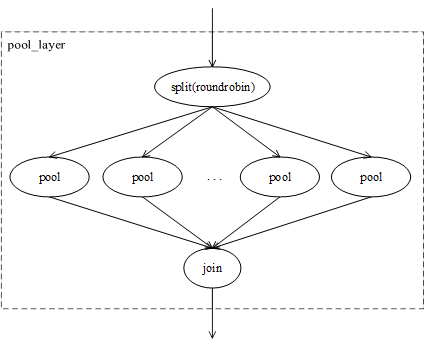
\includegraphics[width=0.5\textwidth]{../img/Chap_Application/Yu/cnn_pooling_layer.png}
\caption{池化层模块中composite间的结构关系示意图}
\label{fig:cnn_pooling_layer}
\end{figure}

\item 卷积与全连接过渡模块

卷积与全连接过渡模块充当全连接层的输入层,模块只负责将最后一层卷积层的输出结果转发给下层全连接层,同时记录此输出结果至全局区域供反向传播时第一层全连接层参数梯度的计算使用。

\item 全连接模块

全连接模块同本小节第一部分所述的全连接神经网络中的隐藏层模块基本相同,其中包含了两个全连接层,每个全连接层有20个节点,每一层的层composite都通过splitjoin的duplicate调用方式完成层内各composite节点的add操作,同时传入index参数确定节点的weight、bias参数在全局区域的位置,传入size参数确定节点composite一次运行所需的数据量。层内的composite负责对输入加权求和并用Sigmoid激励函数激励。

\item 输出层模块

输出层模块上层与全连接模块相连,负责输出0到9十个数字的预测概率值,所以输出层模块内的输出层有十个输出节点,每个节点输出一个数字的预测概率值。具体操作同全连接层一样,都是以splitjoin的duplicate调用进行层内节点composite的add操作。调用时需要给节点composite传入index参数和size参数,为其提供全局区域参数位置和待处理数据的大小。

\item 正反向传播过渡模块

正反向传播过渡模块连接的是正向全连接层和反向全连接层,该模块负责计算出基于均方差损失函数得出的输出值与实际label目标值相减后所得的误差值,因此构造一个diff composite节点即可满足要求,调用此composite节点时需要传入与上层节点输出值大小一致的size参数,即label目标值维数,同时该节点输出值的数量也和label目标值维数一致。
\end{enumerate}

由于反向传播过程在对卷积层各个卷积核以及全连接层各个节点的参数梯度计算时,依赖于当前卷积层或全连接层所对应层的输入数据,所以卷积层模块、池化层模块和全连接模块的各层在正向传播时都在程序的全局区域中保存了临时的输出结果,其中卷积层模块和全连接层模块需要记录的是该层未通过激励函数激励的输出值,和已通过激励函数激励的激励值。由于池化层模块中仅存在池化操作,且池化结果不需要激励函数的激励处理,因此该层只需记录经过池化后的输出值。

LeNet-5卷积神经网络反向传播过程包括七个模块,分别是反向输出层模块、反向全连接模块、反向全连接卷积过渡模块、反向卷积层模块、反向卷积核梯度合并模块、反向池化层模块和参数更新模块。反向传播时,误差以参数梯度的形式在各层间传播,同本小节第一部分所述的全连接神经网络的反向传播过程一样,记损失函数对该层输出值的偏导数为$\delta$,若已知卷积层的$\delta$值,则该层中的各卷积核组的bias偏置参数的梯度等于相对应的$\delta$矩阵的各元素之和,组内各卷积核的weight权重参数的梯度等于该卷积层输入值与$\delta$值经卷积后的结果,因此反向传播时反向卷积层可以通过$\delta$值计算该层参数的梯度。

现考虑已知第m层卷积层的$\delta _{m}$如何计算出上一层第m-1层的池化层所需的$\delta _{m - 1}$,为了计算这个$\delta _{m - 1}$,需要利用复合函数求导的链式法则进行分析,记本层输出值为$Z _{m}$,上层池化层的输出值为$Z _{m - 1}$,卷积核weight权重参数为W,W的转置为$W ^{T}$,则$\delta _{m - 1}$等于将$\delta _{m}$用零扩展得到的矩阵与$W ^{T}$卷积运算再同$Z _{m - 1}$做Hadamard积运算后的结果。再考虑已知第m-1层的池化层的$\delta _{m - 1}$,如何计算出上层第m-2层的卷积层所需的$\delta _{m - 2}$值,由于采用的是2×2最大池化的方式进行池化,反向传播时池化层的$\delta _{m - 1}$的必须要经过上采样还原成池化层输入值的大小,同时由于第m-2层卷积层的卷积结果被ReLU激励函数激励过,记ReLU对x的导数为R(x),第m-2层卷积层的卷积结果为$Z _{m - 2}$,则$\delta _{m - 2}$等于还原后的值与R($Z _{m - 2}$)做Hadamard积运算的结果。以上就是反向传播时,卷积层计算对上层池化层$\delta$和池化层计算上层卷积层$\delta$的过程。以数据流编程模型的角度考虑,$\delta$就是LeNet-5卷积神经网络在反向传播阶段各层间流动的值。

\begin{enumerate}

\item 反向输出层模块

反向输出层模块接收正反向过渡模块的输出值,该模块由反向输出层bout\_layer composite和层内节点bout composite两个composite构成,bout\_layer composite以splitjoin的roundrobin调用方式,将传入的误差值以带index参数的方式分批传给bout composite,bout composite内部计算对应输出层节点的weight和bias参数梯度值,并传出计算完毕的bias梯度值作为下一模块的输入。

\item 反向全连接模块

反向全连接模块中有两个反向全连接层,每层都有各自的bfullconn\_layer composite和节点bfullconn\_node composite,其中bfullconn\_layer composite以splitjoin的duplicate调用方式,复制传入的全部数据给层内的20个bfullconn\_node composite,bfullconn\_node composite计算各节点对应的weight参数和bias参数梯度。

\item 反向全连接卷积过渡模块

由于反向全连接层中各层间传递的是本层的$\delta$值,传入到上层后由上层负责计算上层自己的$\delta$值,而反向卷积层和反向池化层之间传递的是已经在本层计算完毕的上层$\delta$值,因此需要一个过渡层完成这种差异的转变。反向全连接卷积过渡层模块只完成计算与全连接层相连的卷积层的$\delta$值的任务,因此只用一个bconv\_fconn composite完成这个过程。

\item 反向卷积层模块

反向卷积层模块中的各个卷积层有三个任务要处理,分别是计算当前卷积层组的bias参数梯度、计算当前卷积层的组内各通道卷积核的weight参数梯度以及计算反向池化层的$\delta$值。这三个任务之间没有数据依赖关系,因此模块中的bconv\_layer composite以splitjoin的roundrobin调用方式,将每组卷积核对应的$\delta$数据切割后分批传给各个bconv\_group composite。bconv\_group composite在内部以splitjoin的duplicate调用方式,将每组对应的$\delta$数据重复分发给bconv\_bias composite、bconv\_weight composite和bconv\_delta composite三种任务composite,三种任务composite分别负责bias参数梯度的计算、weight参数梯度的计算和$\delta$值的计算,由于只有$\delta$值需要传出,因此bconv\_bias composite和bconv\_weight composite只需要传递一个代表任务完成的信号数据给join节点,bconv\_delta composite则要传递计算出的反向池化层的$\delta$值。

\item 反向卷积核梯度合并模块

反向卷积核梯度合并模块接收反向卷积模块的输出,其中前两个数据是信号数据,处理时直接舍去,其余数据是反向池化层的$\delta$值。由于反向卷积层模块是以分组的形式在各组内计算自己组对反向池化层的$\delta$值,因此需要将各组间相同通道对应的$\delta$值相加,合并成最终的$\delta$值。此模块中包括两个composite,一个是merge\_group composite,负责以splitjoin的roundrobin调用形式提取各卷积组相同通道的输出数据,传入对应的merge composite,每个merge composite完成一个通道的$\delta$值合并操作,合并完成后通过join节点连接合并值再传递给反向池化层模块。

\item 反向池化层模块
 
反向池化层模块只负责用传入的反向池化层$\delta$值计算传入下一反向卷积层$\delta$值,计算需要先对池化层$\delta$值进行上采样操作再乘上卷积时ReLU激励函数对卷积层卷积结果的导数,$\delta$的各通道值在进行次操作时可以同时进行,因此本模块包括pool\_layer composite和pool composite两个composite结构,pool\_layer composite利用splitjoin的roundrobin调用提取各通道的$\delta$值传递给各通道对应的pool composite,pool composite在内部实现对$\delta$值的具体操作。

\item 参数更新模块

参数更新模块负责在一次完整的正向传播和反向传播执行完毕后,对全局区域中卷积核的weight参数、卷积组的bias参数以及全连接层节点的参数进行梯度下降更新,同时参数更新前需要计算实际的改变量,若所有参数的改变量小于某一指定值,则停止模型的训练。

\end{enumerate}

\subsection{相关工作}

\subsection{参考文献}
[1]魏海涛. 面向多核处理器的数据流程序编译关键技术研究(博士论文), 华中科技大学,2010.\\

[2] 张维维, 魏海涛, 于俊清, 李鹤, 黎昊, 杨秋吉. COStream:一种面向数据流的编程语言和编译器实现, 计算机学报, 2013, 36(10):1993 -2006

[3] Haitao Wei, Mingkang Qin, Junqing Yu, Dongrui Fan and Guang R. Gao. StreamTMC: Stream Compilation for Tiled Multi-core Architectures, Journal of Parallel and Distributed Computing (JPDC), 2013, 73(4): 484-494

[4] Haitao Wei, Junqing Yu, Huafei Yu, Mingkang Qin and Guang R. Gao. Software Pipelining for Stream Programs on Resource Constrained Multi-core Architecture, IEEE Transactions on Parallel and Distributed Systems, 2012, 23(12): 2338-2349

[5] Haitao Wei, Junqing Yu, Huafei Yu, Guangrong Gao. Minimizing Communication in Rate-Optimal Software Pipelining for Stream Programs, The 8th International Symposium on Code Generation and Optimization (CGO), 2010,Toronto, Canada, 210~217

[6] 魏海涛, 秦明康, 于俊清,范东睿. 一种面向众核架构的数据流编译框架, 计算机学报, 2014, 37(7): 1560-1569)

[7] 于俊清, 余华飞, 魏海涛, 秦明康. 多核环境下编译器辅助消息驱动的动态调度, 计算机学报, 2014, 37(7): 1633-1637

[8] 于俊清, 张维维, 陈文斌, 涂浩, 何云峰. 面向多核集群的数据流程序层次流水线并行优化方法研究, 计算机学报, 2014, 37(10): 2071-2083

[9] 魏海涛, 于俊清, 余华飞, 秦明康. 一种面向数据流程序的软件流水并行化方法, 计算机学报, 2011, 34(5): 889~898)

[10] 陈文斌,杨瑞瑞,于俊清. 基于GPU/CPU混合架构的流程序多粒度划分与调度方法研究, 计算机工程与科学,2017, 39(1): 15-26)

[11] 杨胜哲, 于俊清, 唐九飞. 数据流程序动态调度与优化方法研究, 计算机工程与科学,2017, 39(7): 1201-1210)

[12] 唐九飞, 李 鹤, 于俊清. 面向X86多核处理器的数据流程序任务调度与缓存优化, 中国科学技术大学学报, 2016, 46(3): 200-207

[13] 王兆吉. 利用COStream实现全连接和卷积神经网络的并行计算(硕士论文),2019,华中科技大学